\documentclass[12pt,a4paper]{report}

%\setlength{\parskip}{\baselineskip}%
%\setlength{\parindent}{0pt}%

\usepackage[utf8]{inputenc}
\usepackage{tabto}

%\usepackage[paperwidth=17cm, paperheight=24cm]{geometry}

%indent lists
\usepackage{enumitem}

\usepackage{amsmath}

\usepackage{hyperref}
\hypersetup{
   colorlinks,
   citecolor=black,
   filecolor=black,
   linkcolor=black,
   urlcolor=black
}

\usepackage{fancytabs}
%variable for fancytabs spacing
\newcommand{\tabSpace}{0.85}

\usepackage[font=footnotesize,labelfont=bf]{caption}
\usepackage[sort,comma]{natbib}
\usepackage{epigraph}
\setlength\epigraphwidth{.8\textwidth}
\setlength\epigraphrule{0pt}
\usepackage{pbox}
\usepackage{graphicx}
\usepackage{pdfpages}
\graphicspath{ {image/} }
\usepackage{epstopdf}
\usepackage{bibentry}
%tells bibentry to (re)use the bibliographic data from the standard BibTeX setup
\nobibliography*

%\usepackage[resetlabels]{multibib}
%\newcites{bibliography/reference}{test}

%abbreviations
%\usepackage[refpage]{nomencl}
%\makenomenclature

% Load the package with the acronym option
\usepackage[acronym,nomain,nonumberlist]{glossaries}
 
% Generate the glossary
\makeglossaries

%scientific notation
%http://www.tapdancinggoats.com/easy-scientific-notation-in-latex.htm
\providecommand{\e}[1]{\ensuremath{\times 10^{#1}}}

\begin{document}

\begin{titlepage}
   \begin{center}
      VRIJE UNIVERSITEIT

      \vspace{1.5cm}

      \fontsize{17}{1em}\selectfont \textbf{High-throughput transcriptome sequencing: methods development and data analysis of large expression data sets}

      \vspace{3cm}

      \fontsize{11}{1em}\selectfont
ACADEMISCH PROEFSCHRIFT

      \vspace{8mm}

ter verkrijging van de graad Doctor aan \\
de Vrije Universiteit Amsterdam, \\
op gezag van de rector magnificus \\
prof.dr. F.A. van der Duyn Schouten, \\
in het openbaar te verdedigen \\
ten overstaan van de promotiecomissie \\
van de Faculteit der Aard- en Levenswetenschappen \\
op maandag 28 september 2015 om 13.45 uur \\
in de aula van de universiteit, \\
De Boelelaan 1105 \\

      \vfill

      \normalsize
      door \\

      \fontsize{16}{2em}\selectfont \textbf{Dave Ting Pong Tang} \\
      \normalsize
      \vspace{1mm}
      geboren te Hong Kong

   \end{center}
\end{titlepage}

\fontsize{13}{1.5em}\selectfont
\noindent
promotor: prof.dr. A.B. Smit \\
copromotor: dr. P. Carninci

\newpage

{
   \setlength{\parindent}{0cm}
   Thesis committee:
   \\
   \\
   prof.dr. J. Heringa \\
   prof.dr. S. Linnarson \\
   prof.dr. A. Sandelin \\
   prof.dr. P.A.C. 't Hoen \\
   dr. K. Bossers \\
}

\newpage

\normalsize
{
   \setlength{\parindent}{0cm}
   The work in this thesis was carried out in the Transcriptome Technology Team in the Division of Genomic Technologies in the RIKEN Center for LifeScience Technologies at the RIKEN Yokohama Institute in Japan and was primarily supported by the EU-ITN BrainTrain program.
   \\
   \\
   About the cover: the cover was generated using R and the Gviz package. Code used to generate the image can be found at \href{http://davetang.org/muse/2015/02/06/thesis-cover-art/}{http://davetang.org/muse}.
   \\
   \\
   Printed by:
   \\
   \\
   ISBN:
   \\
   \\
   All rights reserved. No part of this thesis may be reproduced, stored in a retrieval system, or transmitted in any form or by any means without permission from the author.
}

\chapter*{English Summary}
\small
This thesis is on the use of DNA sequencing to investigate the transcriptome, which is the complete set of transcripts in a cell. Technologies for the interrogation of nucleic acids have made it possible to investigate different biological questions.


\chapter*{Nederlandse Samenvatting}
Recente ontwikkelingen op het gebied van DNA sequentie analyse hebben geleid tot zogenaamde ``high-throughput sequencing". Dit heeft DNA sequentie analyse mogelijk gemaakt die zowel tijds- als kostenbesparend werkt.

Met het gereedkomen van de sequentie van het humane genoom en de sequentie van de genomen van andere species, is de nadruk bij genoom sequentie analyse komen te liggen op de identificatie van kleine functionele elementen in het DNA.  Het veld van transcriptoom analyse heeft zich voornamelijk gericht op de correcte annotatie en data analyse van de getranscribeerde producten. De introductie van high-throughput sequencing in transcriptoom analyse heeft een unbiased en accurate screening van het transcriptoom mogelijk gemaakt, en heeft daarmee inzicht geboden in de grote complexiteit van bijvoorbeeld het humane genoom. Echter alle methoden zijn nog relatief nieuw en niet gematureerd, eigenlijk allemaal ontwikkeld in de laatste 5-6 jaar. Daarom vinden er continu verbeteringen aan deze methoden plaats. In mijn dissertatie besteed ik daarom veel aandacht aan het gebruik van bio-informatica methoden om het transcriptoom beter te kunnen analyseren.

In hoofdstuk 2 richt ik mij daarom op de mogelijke bias en technische artefacten  die bij de transcriptoom analyse voor kunnen komen, in het bijzonder die bij de ``nano-CAGE" analyse kunnen optreden. In het bijzonder vond ik artefacten die werden geintroduceerd door het gebruik van moleculaire barcodes en ik heb verschillende methoden ontwikkeld om hier om op een juiste wijze mee om te gaan.

In hoofdstuk 3 heb ik mij gericht op het analyseren van het transcriptoom van cellen met geinduceerde DNA schade gebruik makend van sequentie analyse van ``small RNAs". Hierbij ontdekten we een nieuwe vorm van RNA molekulen, die worden gevormd dicht op de plaatsen van DNA schade. Deze RNAs vormen de respons op de DNA schade.

In hoofdstuk 4 heb ik de expressie van een specifieke klasse van ``small RNAs" bestudeerd, de zogenaamde Piwi-interacterende RNAs (piRNAs). Dit werd gedaan in muizen met een deletie van het Mecp2 gen. Onze analyse liet zien dat piRNAs tot overexpressie komen in het cerebellum van muizen met een Mecp2 deletie, hetgeen te maken kan hebben met de voorgestelde rol van Mecp2 in het silencen van transposons.

In hoofdstuk 5 heb ik me gericht op het bestuderen van transcripten die ontstaan uit repetitieve elementen (RE) in het DNA. Ik heb daarbij het expressie profiel van deze transcripten voor een groot aantal cellijnen, weefsels, en primaire cellen in kaart gebracht. Ik heb daaruit geconcludeerd dat RE's belangrijk zijn voor de expressie van de ``long non-coding RNAs" en ``enhancer RNAs", waarbij hun expressie weefsel specifiek is.

In conclusie, high-throughput sequentie analyse heeft het veld van transcriptoom analyse wezenlijk veranderd door veel meer complexiteit van transcriptie aan te tonen dan daarvoor voor mogelijk werd gehouden. De lagen van complexiteit die we daarbij hebben ontdekt omvatten meerdere klassen van RNA's, ieder met een eigen regulatoire rol, random transcriptionele gebeurtenissen ook wel ``random noise" genoemd, en inzicht in de complexiteit van de technische artefacten. Het scheiden van technische variatie van het echte signaal vergt begrip van de verschillende technologieen, diepgaande data analyse, en de ontwikkeling van adequate bio-informatische methoden.

\normalsize

\chapter*{List of publications}

\begin{enumerate}
   \item \bibentry{Tang01022013}
   \item \bibentry{francia2012site}
   \item \bibentry{saxena2012pirnas}
   \item \bibentry{fantom5repeat}
\end{enumerate}

\section*{Other publications}

\begin{enumerate}
   \setcounter{enumi}{4}
   \item \bibentry{hasegawa2014ccl2}
   \item \bibentry{bloodtranscriptome}
\end{enumerate}

\tableofcontents
\listoffigures
\listoftables

% Acronym definitions
% \newacronym{<label>}{<abbrv>}{<full>}

\newacronym{qc}{QC}{Quality control}
\newacronym{cre}{CRE}{Cis-regulatory elements}
\newacronym{rtt}{RTT}{Rett syndrome}
\newacronym{mbd}{MBD}{methyl-CpG binding domain}
\newacronym{mecp2}{MECP2}{methyl CpG binding protein 2}
\newacronym{ridl}{RIDL}{Repeat Insertion Domains of LncRNAs}
\newacronym{rap}{RAP}{Repeat Analysis Pipeline}
\newacronym{fdr}{FDR}{False discovery rate}
\newacronym{tmm}{TMM}{Trimmed mean of M values}
\newacronym{anova}{ANOVA}{Analysis of variance}
\newacronym{page}{PAGE}{Polyacrylamide gel electrophoresis}
\newacronym{solid}{SOLiD}{Sequencing by Oligonucleotide Ligation and Detection}
\newacronym{mecp2}{MecP2}{Methyl CpG binding protein 2}
\newacronym{tbp}{TBP}{TATA binding protein}
\newacronym{rabs}{RABS}{Repeat-associated binding sites}
\newacronym{tuf}{TUF}{Transcripts of unknown function}
\newacronym{trna}{tRNA}{Transfer RNA}
\newacronym{mrna}{mRNA}{Messenger RNA}
\newacronym{rna}{RNA}{Ribonucleic acid}
\newacronym{dna}{DNA}{Deoxyribonucleic acid}
\newacronym{ddr}{DDR}{DNA damage response}
\newacronym{rnapol}{RNA pol}{RNA polymerase}
\newacronym{poli}{Pol I}{RNA polymerase I}
\newacronym{polii}{Pol II}{RNA polymerase II}
\newacronym{poliii}{Pol III}{RNA polymerase III}
\newacronym{bre}{BRE}{B recognition element}
\newacronym{cgi}{CGI}{CpG islands}
\newacronym{cpat}{CPAT}{Coding-potential assessment tool}
\newacronym{rt}{RT}{Reverse transcriptase}
\newacronym{bp}{BP}{Base pair}
\newacronym{dbd}{DBD}{DNA-binding domain}
\newacronym{ccl2}{CCL2}{chemokine (C-C motif) ligand 2}
\newacronym{nacl}{NaCl}{Sodium chloride}
\newacronym{qrtpcr}{qRT-PCR}{Quantitative real-time polymerase chain reaction}
\newacronym{pcr}{PCR}{Polymerase chain reaction}
\newacronym{pet}{PET}{Paired-end ditag}
\newacronym{a}{A}{Adenine}
\newacronym{c}{C}{Cytosine}
\newacronym{g}{G}{Guanine}
\newacronym{t}{T}{Thymine}
\newacronym{u}{U}{Uracil}
\newacronym{ipsc}{iPSC}{Induced pluripotent stem cell}
\newacronym{asc}{ASC}{Adult stem cell}
\newacronym{esc}{ESC}{Embryonic stem cell}
\newacronym{cage}{CAGE}{Cap analysis gene expression}
\newacronym{nanocage}{nanoCAGE}{Nano Cap analysis gene expression}
\newacronym{sage}{SAGE}{Serial analysis gene expression}
\newacronym{cdna}{cDNA}{Complementary DNA}
\newacronym{chip}{ChIP}{Chromatin immunoprecipitation}
\newacronym{encode}{ENCODE}{Encyclopedia of DNA elements}
\newacronym{fantom}{FANTOM}{Functional annotation of the mammalian genome}
\newacronym{go}{GO}{Gene ontology}
\newacronym{lncrna}{lncRNA}{Long non-coding RNA}
\newacronym{ncrna}{ncRNA}{Non-coding RNA}
\newacronym{mirna}{miRNA}{Micro RNA}
\newacronym{primirna}{pri-miRNA}{Primary miRNA}
\newacronym{premirna}{pre-miRNA}{Precursor miRNA}
\newacronym{pirna}{piRNA}{Piwi-interacting RNA}
\newacronym{pirisc}{piRISC}{piRNA-induced silencing complex}
\newacronym{tf}{TF}{Transcription factor}
\newacronym{tu}{TU}{Transcriptional unit}
\newacronym{tfiib}{TFIIB}{Transcription factor IIB}
\newacronym{tfbs}{TFBS}{Transcription factor binding site}
\newacronym{tss}{TSS}{Transcription start site}
\newacronym{re}{RE}{Repetitive elements}
\newacronym{te}{TE}{Transposable element}
\newacronym{line}{LINE}{Long interspersed elements}
\newacronym{sine}{SINE}{Short interspersed elements}
\newacronym{ltr}{LTR}{Long terminal repeat}
\newacronym{erv}{ERV}{Endogenous retrovirus}
\newacronym{rt}{RT}{Reverse transcriptase}
\newacronym{ts}{TS}{Template switching}
\newacronym{3d}{3D}{Three-dimensional}
\newacronym{hgp}{HGP}{Human genome project}
\newacronym{sam}{SAM}{Sequence alignment/map}
\newacronym{sbl}{SBL}{Sequencing by ligation}
\newacronym{sbs}{SBS}{Sequencing by synthesis}
\newacronym{crt}{CRT}{Cyclic reversible termination}
\newacronym{sna}{SNA}{Single-nucleotide addition}
\newacronym{empcr}{emPCR}{Emulsion PCR}
\newacronym{ddntp}{ddNTP}{Dideoxynucleotide triphosphate}
\newacronym{datp}{dATP}{Deoxyadenosine triphosphate}
\newacronym{dctp}{dGTP}{Deoxycytidine triphosphate}
\newacronym{dgtp}{dCTP}{Deoxyguanosine triphosphate}
\newacronym{dttp}{dTTP}{Deoxythymidine triphosphate}

%Print the entire glossary
\glossarystyle{long}
\glsaddall
\printglossary[title=List of Abbreviations,toctitle=List of Abbreviations]


\chapter{Introduction}\label{intro}
\fancytab{Chapter ~\ref{intro}}{\tabSpace*\thechapter}
\section{History of DNA and genes}

In the winter of 1868/9, Swiss physician and biologist, Johannes Friedrich Miescher isolated an unknown substance from the nuclei of cells\cite{dahm2008discovering}. This substance was unlike anything he had observed before; it was resistant to protease, lacked sulphur, and contained a large amount of phosphorous. He recognised that he had isolated a novel substance and as it was from the nucleus, he named it nuclein. In 1881, Albrecht Kossel determined that nuclein was composed of five bases: adenine (A), cytosine (C), guanine (G), thymine (T), and uracil (U). Later in 1889, Richard Altmann discovered that nuclein was acidic (due to presence of phosphorous) and renamed nuclein to nucleic acid. The basic component of deoxyribonucleic acid (DNA) was deduced by Phoebus Levene in 1909, where he discovered that DNA consisted of an acid, an organic base, and a sugar. Levene also showed that these components were linked together as phosphate-sugar-base to form units, which he termed nucleotides. This sugar-phosphate backbone forms the structural framework of nucleic acids and makes DNA highly stable. In 1928, Frederick Griffith demonstrated that heritable traits could be transferred between dead and live bacteria and that provided the first clue that a ``transforming factor" existed\cite{griffith1928significance}. It wasn't until 1944, when Oswald Avery, Colin MacLeod, and Maclyn McCarty demonstrated that deoxyribonucleodepolymerase (an enzyme that degrades DNA) destroyed the ``transforming factor", that it was hypothesised DNA was the genetic material\cite{avery1944studies}. This was later confirmed in 1952 by Alfred Hershey and Martha Chase, by demonstrating that when bacteriophages infected bacteria, only their DNA would enter into the cytoplasm of the bacteria, while their protein remained outside\cite{hershey1952independent}.

While Phoebus Levene proposed that DNA was made up equal amounts of A, C, G, and T, it was later discovered by Erwin Chargaff that DNA should have a 1:1 ratio of pyrimidine (C, T, and U) and purine (A and G) bases\cite{pmid14938364, pmid14945441}; this became known as Chargaff's rules. The three-dimensional (3D) structure of DNA was solved by Francis Crick and James Watson in 1953\cite{WATSON_1953} after gaining insight from an X-ray diffraction image taken by Rosalind Franklin and from Chargaff's rules. The 3D structure of DNA showed how adenines paired with thymines and cytosines paired with guanine (Figure ~\ref{fig:dna}). The base pairing, now known as Watson-Crick base pairing, explained how genetic information could be copied.

\begin{figure}[!ht]
   \centering
   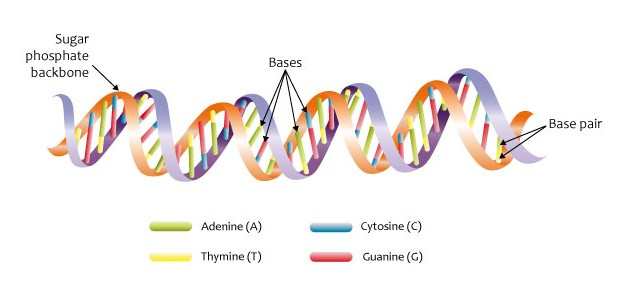
\includegraphics[width=\textwidth,natwidth=625,natheight=307]{dna.jpg}
   \caption[The structure of DNA]{The structure of DNA is based on the repeated pattern of a sugar and phosphate group, known as the sugar phosphate backbone, and the base pairing of the four bases, adenine (A), cytosine (C), guanine (G), and thymine (T). Image by NHS National Genetics and Genomics Education Centre licensed under the Creative Commons license.}
   \label{fig:dna}
\end{figure}

The definition of a gene has evolved with our increasing knowledge of genetics and biochemistry\cite{pmid17567988}. The idea of a gene dates back to Gregor Mendel when he demonstrated in his plant breeding experiments that discrete traits could be inherited from parents to offspring. While the mechanism of inheritance was not clear at that time, these heritable traits became known as a gene. In 1941, George Beadle and Edward Tatum observed that mutations in Neurospora genes would cause defects in steps of a metabolic pathways\cite{Beadle15111941}. The demonstration of how genes directed the synthesis of enzymes later became known as the ``one gene, one polypeptide" hypothesis, where each gene was responsible for producing a single protein in a biochemical pathway.

The pathway from genes to proteins was established with the discovery of the ribosomes\cite{pmid14381428}, transfer RNA (tRNA)\cite{pmid13538965}, and messenger RNA (mRNA), which carries the information between a gene and protein\cite{BRENNER1961}. The code used by DNA to encode the amino acids of proteins was demonstrated by the use of artificial ribonucleic acid (RNA) and bacterial cells\cite{pmid14471390}. By using artificially created RNA that composed entirely of uracils, Matthaei and colleagues produced a protein composed entirely of the amino acid phenylalanine. The full code, known as the genetic code, was cracked three years later\cite{pmid5330357} and defined how information is encoded in DNA. Nirenberg and colleauges deduced that three nucleotides defined a codon and is translated into one of the 20 standard amino acids. This flow of information from nucleic acid to protein was described as the ``Central Dogma"\cite{crick1958protein}.

\section{DNA to RNA}

The genome is a store of biological information that requires the coordinated activity of proteins to bring it to life. This is achieved via transcription, which is a highly regulated mechanism that begins with RNA polymerase attaching to DNA and processes the template DNA strand into a single-stranded RNA molecule (Figure ~\ref{fig:transcription}). Transcription results in two main classes of RNA or transcripts: (1) Protein-coding transcripts, where the RNA known as mRNA can be further translated into a protein molecule and (2) Non-coding transcripts, where the RNA molecule is the functional product.

There are three different types of RNA polymerases in eukaryotic cells: Pol I transcribes DNA that encode most of the ribosomal RNAs (rRNAs); Pol II transcribes DNA that encode mRNAs and other non-coding RNAs; and Pol III transcribes the genes for small regulatory RNA molecules, such as transfer RNA (tRNA). RNA polymerase binds upstream of the DNA to be transcribed, at a region known as the promoter. Promoters can be classified by their distance to the transcription start site (TSS), which are the first nucleotides transcribed by RNA polymerase. The core promoter is the closest to the TSS and contains specific DNA sequences or elements that are necessary for transcription. The core promoter elements include the TATA box (usually located 25 to 35 bases upstream of the TSS), the initiator element (Inr), the downstream promoter element (DPE), the TFIIB recognition element (BRE), and CpG islands (CGIs). The proximal promoter lies $\sim~250$ bp of the TSS and contains primary regulatory elements. Distal promoters do not have a fixed distance from the TSS but are usually further upstream and contain additional regulatory elements. Pol I and Pol III transcription are similar, but their promoter sequences and activator proteins differ.

\begin{figure}[!ht]
   \centering
   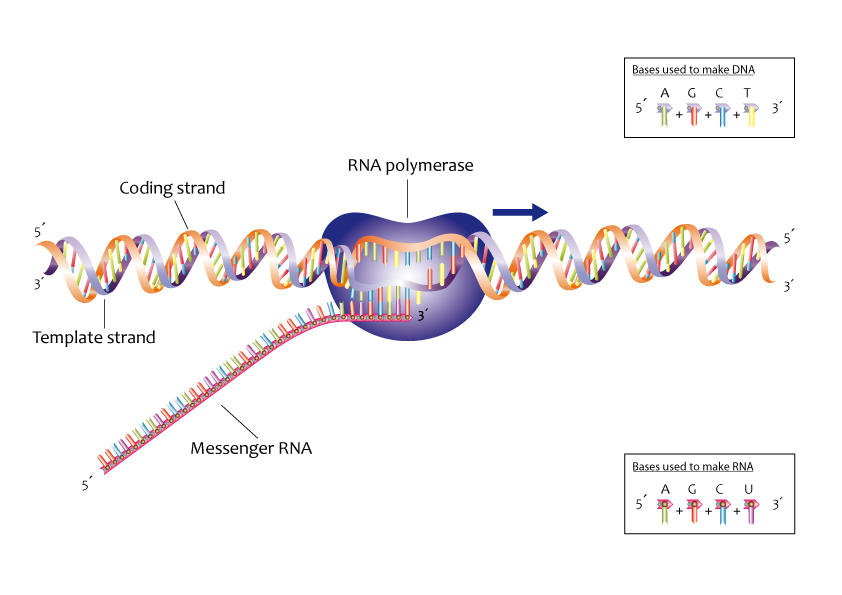
\includegraphics[width=\textwidth,natwidth=842,natheight=595]{transcription.jpg}
   \caption[DNA transcription]{The process of transcription when the DNA double helix unwinds and the RNA polymerase reads the DNA sequence (the template strand) in the 5' to 3' direction and produces a complementary RNA strand called the messenger RNA (mRNA). The mRNA has the same sequence as the coding strand, except that thymines are replaced by uracils. Image by NHS National Genetics and Genomics Education Centre licensed under the Creative Commons license.}
   \label{fig:transcription}
\end{figure}

\subsection{Transcription factors}

Transcription factors (TFs) are regulatory proteins that can activate or enhance the transcription of DNA by binding to specific DNA sequences at promoters (they are also known to negatively regulate transcription but this is less common)\cite{pmid11092823}. TFs contain one or more DNA-binding domains that allow it to bind to specific DNA sequences. For example, the TATA binding protein (TBP), which is known as a general transcription factor (GTF), binds to the TATA box and is involved in DNA strand separation during transcription. Other GTFs include TFIIA, TFIIB, TFIID, TFIIE, TFIIF, and TFIIH, and are necessary components of transcription. Not all the GTFs bind to DNA but they are part of the large transcription preinitiation complex (PIC) that interacts with RNA polymerase and helps position it over the TSS. The DNA sequence that TFs bind to is called the transcription factor binding site (TFBS), however a single TF can bind to different DNA sequences that are similar. As such, TFBSs are represented as sequence logos, i.e. a consensus sequence, which are built from a collection of aligned sequences that the TF bound to. Mutations in TFs can cause disease, for example, mutations in the methyl CpG binding protein 2 (MECP2) gene is the cause of most cases of Rett syndrome.

\subsection{Post-transcriptional modifications}

The termination of transcription relies on terminator sequences that are found close to the ends of transcripts. For Pol I transcripts, transcription is stopped by a termination factor that unwinds the DNA-RNA hybrid formed during transcription. For Pol III transcripts, inverted repeats are transcribed and these sequences can form hairpin loops that pauses the RNA polymerase. For Pol II transcripts, a polyadenylation signal (AAUAAA) at the end of the sequence is necessary for termination\cite{pmid3479794}. The nascent RNA is cleaved at the polyadenylation site and a poly-adenine tail (poly(A)) is added; the poly(A) tail is important for the stability of the RNA, translation, and for nuclear export. Other post-transcriptional modifications include a specialised nucleotide cap that is added to the 5' end, which is recognised by the ribosomes during protein synthesis. The ribosome binds to the cap and reads along the 5' untranslated region (UTR) until it reaches an initiation codon. Removal of the cap is considered as the first step towards mRNA degradation. The capping procedure is thought to occur only in the nucleus, however a cytoplasmic capping enzyme has been identified\cite{pmid22921400}.

\section{DNA packaging}

The default state of transcription in eukaryotes is that most genes are not constantly transcribed due to structural properties of DNA that make it inaccessible to the PIC. DNA is packed into chromosomes, which are long DNA molecules that are condensed, enabling DNA to physically fit inside the nucleus (Figure ~\ref{fig:dna_condensed}). Histones, which are a family of small and positively charged proteins, provide the energy, in the form of electrostatic interactions, to fold negatively charged DNA (due to the phosphate groups in its phosphate-sugar backbone). This folding helps condense the DNA and the resulting DNA-protein complex is called chromatin.

Chromatin possesses a fundamental repeating structure\cite{holde01111974}, known as nucleosomes and the packaging of DNA into nucleosomes shortens DNA about sevenfold. However despite this, chromatin is still too long to fit inside the nucleus, which is approximately 10 to 20 microns in diameter. Chromatin is further coiled into a thicker fiber, called the 30nm fiber, because it is roughly 30 nanometers in diameter. Processes such as transcription and replication require the two strands of DNA to come apart temporarily, thus allowing polymerases access to the DNA template. However, the presence of nucleosomes and the folding of chromatin into 30-nanometer fibers pose barriers to the enzymes that unwind and copy DNA. It is therefore important for cells to have means of opening up chromatin fibers and/or removing histones transiently to permit transcription and replication to proceed.

The core histones are H2A, H2B, H3, and H4 and they 

Chromatin structure and nucleosome positioning are altered in order for the transcriptional machinery to access parts of the genome for transcription.

\begin{figure}[!ht]
   \centering
   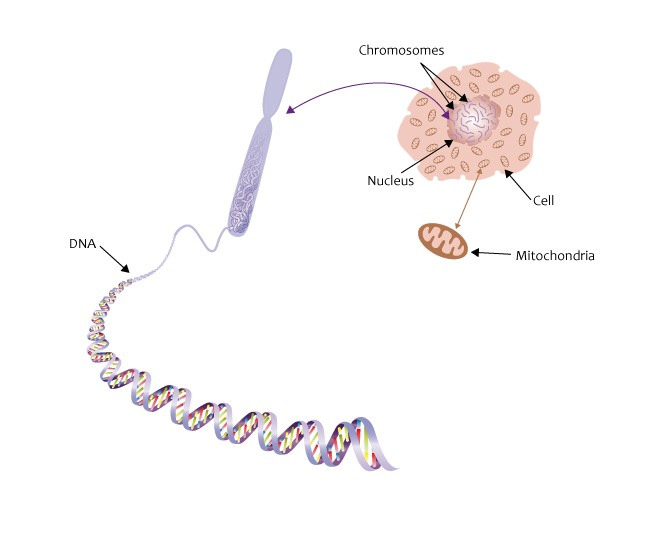
\includegraphics[width=\textwidth,natwidth=650,natheight=539]{dna_condensed.jpg}
   \caption[Condensation of DNA]{DNA is condensed into chromosomes by forming DNA-protein complexes known chromatin, which is further coiled into thicker fibers called 30nm fibers. The chromosomes reside inside the nucleus of a cell. Mitochondria also contain its own DNA. Image by NHS National Genetics and Genomics Education Centre licensed under the Creative Commons license.}
   \label{fig:dna_condensed}
\end{figure}


\subsection{Histone modifications}

Generally speaking, there are two major mechanisms by which chromatin is made more accessible:

\begin{enumerate}
   \item Histones can be enzymatically modified by the addition of acetyl, methyl, or phosphate groups.
   \item Histones can be displaced by chromatin remodelling complexes, thereby exposing underlying DNA sequences to polymerases and other enzymes.
\end{enumerate}

These two processes are reversible, so modified or remodelled chromatin can be returned to its compact state after transcription and/or replication are complete. The common nomenclature of histone modifications is by the name of the histone (e.g. H3), the single-letter amino acid abbreviation (e.g. K for lysine) and its position (e.g. 27), and the type of enzymatic modification (e.g. acetylation); put together this is represented as H3K27ac. Specific histone modifications are linked to different biological states; for example, acetylation removes the positive charge on the histones, decreasing the interaction between histones and DNA, leading to transcriptional activation. On the other hand, the tri-methylation of lysine 27 on histone H3, i.e., H3K27me3, is associated with the inhibition of transcription\cite{pmid21652639}. Given that distinct histone modifications can either activate or repress transcription, a ``histone code" has been proposed\cite{pmid11498575} and the profiling of the histone states will provide clues to the transcriptional state of a DNA region.

\section{DNA sequencing}

The process of DNA sequencing is the determination of the exact order of nucleotides within a DNA molecule. The first generation of DNA sequencing methods consisted of the electrophoretic methods (Sanger and Maxam-Gilbert sequencing), which were very labour intensive, requiring 4 separate reactions for the determination of each base. One of the first innovations was the use of different fluorophores with Sanger sequencing, which allowed the reactions to be pooled together during gel electrophoresis and eliminated the use of radioactive material. Automation of the DNA sequencing process was possible with the development of an apparatus that could detect the fluorescence emitted by the chain terminated fragments. This development was key towards the success of the Human Genome Project (HGP). For over 25 years since its inception, Sanger sequencing was the method of choice for DNA sequencing.

\subsection{Sanger and Maxam-Gilbert sequencing}

Sanger sequencing\cite{pmid271968} and Maxam-Gilbert sequencing\cite{pmid265521} were two methods of DNA sequencing developed in the 1970s requiring the use polyacrylamide gel electrophoresis, which allowed the resolution of DNA fragments at a 1 bp resolution, and allowed the determination of the DNA bases. The key feature of Sanger sequencing is the use of dideoxynucleotide triphosphates (ddNTPs) and a purified DNA polymerase enzyme to synthesise DNA. The structure of a normal nucleotide (dNTP), consists of a 3' hydroxyl (OH) group in the pentose sugar. The chain-terminating ddNTPs lack the OH group that is necessary for the formation of the phosphodiester bond between one nucleotide and the next during DNA strand elongation. If a ddNTP is incorporated into a growing DNA strand, the strand elongation is terminated. The idea is to set up a reaction with a mixture of dNTPs [deoxyadenosine triphosphate (dATP), deoxyguanosine triphosphate (dGTP), deoxycytidine triphosphate (dCTP), deoxythymidine triphosphate (dTTP)] and one particular ddNTP in a ratio of 300:1. Most of the times, the DNA will be elongated but once the ddNTP is incorporated the strand stops. This results in a number of DNA fragments of varying lengths and depending on the ddNTP used, the last base of the fragment corresponds to that base. This reaction is carried out for the other ddNTPs and all the fragments are separated using polyacrylamide gel electrophoresis. By reading the ladder, the DNA bases can be deduced. The Maxam-Gilbert sequencing method relies on the use of chemicals that can cleave specific bases. Dimethyl sulfate is used to cleave purine bases (A and G) and hydrazine is used to cleave pyrimidine bases (C and T). To distinguish the purines, an adenine-enhanced cleavage step is carried out, which cleaves adenines preferentially. To distinguish the pyrimidines, NaCl is used with hydrazine to suppress the reaction of thymines. As with Sanger sequencing, the DNA fragments are separated using polyacrylamide gel electrophoresis, and the DNA bases are deduced by reading the gel.

Sanger sequencing became the \textit{de facto} method for DNA sequencing due to its comparative ease and the use of fewer toxic materials than Maxam-Gilbert sequencing. A further improvement to Sanger sequencing replaced the need to radioactively label the DNA fragments by using chemically synthesised fluorescent oligonucleotide primers\cite{pmid3713851}. Four different fluorophores were used for each ddNTP reaction allowing all four reactions to be co-electrophoresed and the DNA sequence was deduced by reading the fluorescence colours. The development of a fluorescence detection apparatus linked to a computer that processed the data created the world's first partially automated DNA sequencer\cite{pmid3713851}.

\subsection{Next-generation sequencing}

The next wave of DNA sequencing methods, the so-called next-generation (next-gen) or second generation sequencing, started with various strategies that rely on a combination template preparation, sequencing, and imaging that allowed thousands to billions of sequencing reactions to be performed simultaneously\cite{pmid19997069}. Next-gen sequencing relies on the clonal amplification of templates and use \textit{in vitro} cloning rather than bacterial cloning; the two most common methods are emulsion PCR (emPCR)\cite{pmid12857956} and solid-phase amplification\cite{pmid16473845}. With emPCR individual DNA molecules are isolated with primer-coated beads in water-in-oil microreactors and clonal amplification leads to thousands of copies of the DNA molecule in an emulsion. 454 pyrosequencing and SOLiD sequencing use emPCR, where the amplification product is deposited into individual wells for sequencing. Solid-phase amplification relies on a lawn of high-density primers that are covalently attached on a slide surface (also known as a flow cell) and bind to DNA molecules ligated with sequencing adaptors. The two methods allow each DNA template to be spatially separated, allowing massively parallel sequencing to take place.

Sequencing can take place via the use of DNA polymerase, which is commonly known as sequencing-by-synthesis, and via the use of DNA ligase, known as sequencing-by-ligation (SBL). SBS can be further classified into cyclic reversible termination (CRT), single-nucleotide addition (SNA) and real-time sequencing\cite{pmid19997069}. CRT uses reversible terminators and initial developments used the same dideoxynucleotides used as chain terminators in Sanger sequencing. The concept of CRT is that a DNA polymerase incorporates one fluorescently modified nucleotide, which has a reversible terminator that terminates DNA synthesis. Unincorporated nucleotides are washed away and fluorescence imaging takes place to determine the identity of the incorporated nucleotide. The last step removes or cleaves the reversible terminator and the fluorescent dye and the cycle is repeated. The CRT method is used in Solexa/Illumina and Helicos sequencing. SBL relies on DNA ligase and either one-base-encoded or two-base-encoded probes that are fluorescently labelled. The probes hybridise to its complementary sequence on the primed template and DNA ligase is added to join the probe to the primer. Non-ligated probes are washed away followed by fluorescence imaging and cleavage of the fluorescent dye and the cycle is repeated. The SBL method is used in SOLiD sequencing.

\subsection{Third generation sequencing and beyond}

The third generation of sequencing refers to single-molecule sequencing technologies, which have the capacity for longer read lengths at potentially cheaper costs\cite{pmid20858600}. One of the main advantages of single-molecule sequencing is that PCR is not required, therefore amplification biases and PCR mutations are eliminated. Furthermore, quantitative applications of sequencing such as RNA sequencing are much more representative of the true abundance of RNA molecules. The HeliScope sequencer was the first commercially available single-molecule sequencer, which was based on the work of Stephen Quake and colleagues\cite{pmid12651960}. HeliScope sequencing utilises billions of primed single-molecule templates are covalently attached to the solid support and uses CRT but with slight differences from Solexa/Illumina sequencing. HeliScope uses Helicos Virtual Terminators, which differ from the reversible terminators used in Solexa/Illumina sequencing and dye labelled nucleotides are added individually in the predetermined order of C, T, A, and G, which is followed by fluorescence imaging.

With the advent of next-gen sequencing we have the capacity to sequence an entire human genome in a matter of days. Developments in next-gen sequencing are aiming towards longer read lengths with higher output (Figure ~\ref{fig:dev_next_gen}) and we have just recently arrived in the \$1,000 genome era, whereby we can sequence the entire genome of an individual for around \$1,000 US dollars (USD). In contrast, the Human Genome Project (HGP), which gave us the first glimpse of the human genome\cite{lander2001initial} costed approximately 2.7 billion fiscal year 1991 US dollars\cite{nhgri2010cost}. Next-gen sequencing is also not just limited to genome sequencing; reverse transcriptase\cite{pmid4316300, pmid4316301} allow for the synthesis of complementary DNA (cDNA) from RNA and therefore the entire collection of RNA, known as the transcriptome, can be sequenced. Other applications of next-gen sequencing has allowed us to capture in a genome-wide manner DNA-protein interactions, DNA methylation patterns, and histone modifications\cite{applicationsofsequencing} and the number of protocols utilising next-gen sequencing are continually growing\cite{pachter2014seq}.

\begin{figure}[!ht]
   \centering
   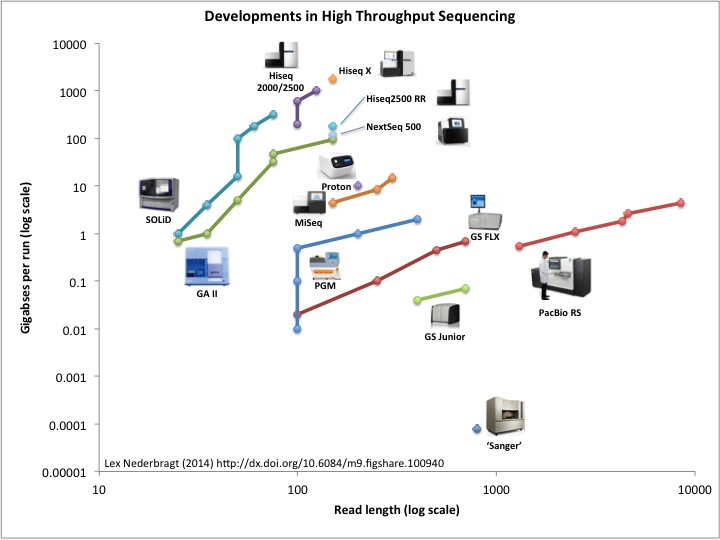
\includegraphics[width=\textwidth,natwidth=720,natheight=540]{developments-in-next-generation-sequencing.jpg}
   \caption[Developments in next generation sequencing]{Log read length versus log gigabases per run for various next generation sequences\cite{Nederbragt2012}.}
   \label{fig:dev_next_gen}
\end{figure}

\section{RNA sequencing}

The transcriptome is the complete collection of RNA molecules in a cell at a specific developmental stage or under a specific physiological condition. The profiling of transcripts or expression profiling reveals the molecular constituents (the RNA and the promoter) that are active under a specific condition and allows the inference of biological pathways and regulatory mechanisms. One of the first technologies that allowed the simultaneous profiling of thousands of transcripts was microarrays\cite{pmid7569999}, which is a hybridization-based approach. Basically, probes that are complementary to specific DNA sequences, such as protein-coding transcripts or genomic regions, are attached to a solid surface. One of the first studies using microarrays showed that the switching from aerobic to anaerobic respiration in yeast changed the levels of over 700 mRNAs by two fold or higher\cite{pmid9381177}. However microarrays have several limitations, which includes \textit{a priori} knowledge of the genome or transcript sequences in order for the probes to be designed, high background levels from cross-hybridisation\cite{pmid16749918}, and a limited dynamic range in expression, which relies on fluorescence signal. 

RNA sequencing (RNA-Seq) is an application of next-gen sequencing used to catalogue the transcriptome as well as quantifying the expression levels of individual transcripts\cite{pmid19015660}. RNA-Seq requires no \textit{a priori} knowledge of the genome, provides a digital gene expression (DGE) profile, and does not suffer from cross-hybridisation issues, which are all limitations of microarrays. RNA-Seq can be applied to total RNA libraries, which sequences the entire population of RNA, or poly-A libraries, which sequences transcripts that have a poly-A tail (mostly mRNAs). A variant of RNA-Seq is small RNA sequencing, which uses size selection to purify RNA that are less than 200 nucleotides, followed by adaptor ligation and sequencing. The sequencing of larger RNA molecules requires an additional fragmentation step, which can introduce biases\cite{pmid18516045}. While RNA-Seq encapsulates all RNA sequencing applications, it is usually associated with the fragmentation of RNA followed by sequencing. There are some protocols that sequence RNA but only the 5'\cite{pmid15300261,pmid14663149} or 3'\cite{pmid22454233} ends of RNA.

While the rate of transcription directly governs the number of transcripts that are present, the stability of transcripts also play a part.

\subsection{Cap Analysis Gene Expression}

Cap Analysis Gene Expression (CAGE) was initially conceived as an idea of profiling all active promoters and TFs for understanding the interplay between the two\cite{carninci2010capanalysis}. CAGE uses a molecular technique known as Cap-Trapper\cite{pmid8938445,pmid9179497}, which allows the capturing of all RNAs that have a cap structure (specifically the diol group of RNA were biotinylated). (Figure ~\ref{fig:cage_protocol}). CAGE allows the genome-wide identification of transcription start sites as well as their expression levels and has been used in various FANTOM projects\cite{pmid16141072, pmid19377474, pmid24670764} and in ENCODE\cite{pmid17571346, pmid22955620}. In the FANTOM3 project, CAGE unveiled the transcriptional landscape in mammalian genomes\cite{pmid16141072} and identified many novel mRNAs and non-coding RNAs not previously characterised and revealed two major classes of promoters: conserved TATA box-enriched promoters and CpG-rich promoters\cite{pmid16645617}. Two variants of CAGE include nanoCAGE\cite{pmid20543846} and HeliScopeCAGE\cite{pmid21596820}. NanoCAGE utilises the template-switching method\cite{pmid11314272} instead of Cap-Trapper and allows for smaller starting amounts of RNA, to the level of RNA content in single cells. HeliScopeCAGE utilises Cap-Trapper but without the enzymatic tag cleavage and PCR amplification, and the capped 5' ends of the cDNA are directly sequenced on the HeliScope sequencer.

\begin{figure}[!ht]
   \centering
   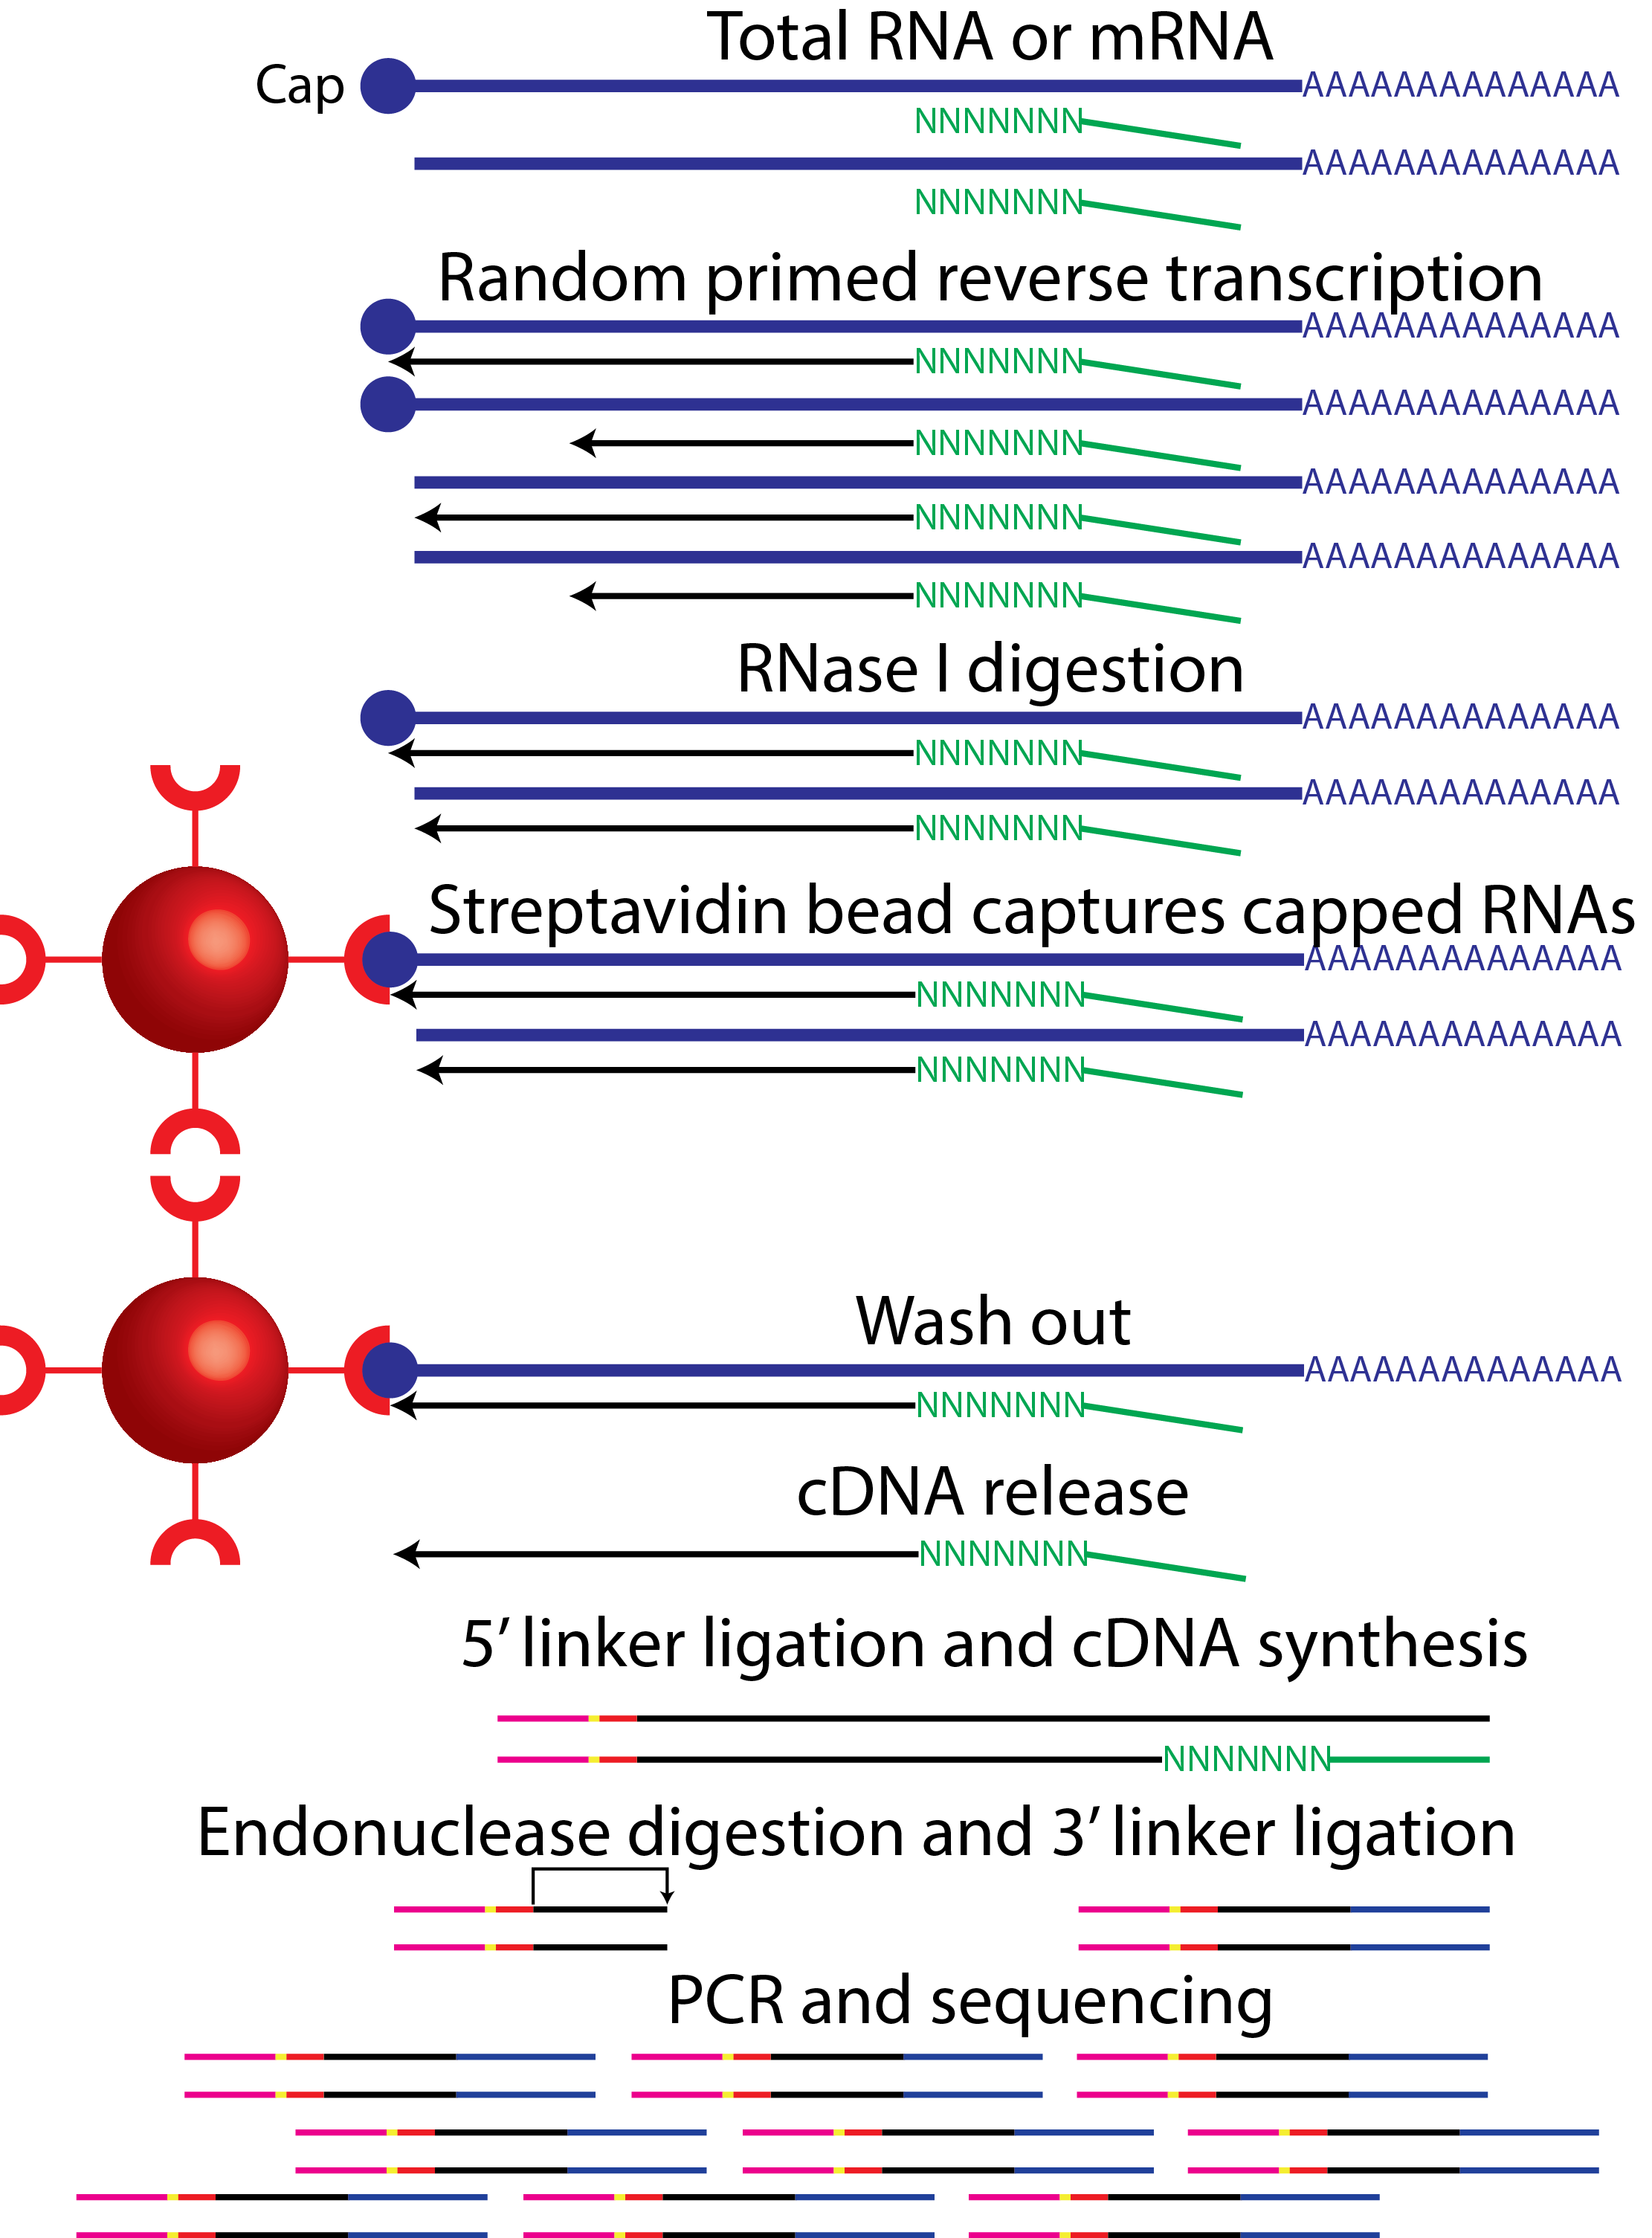
\includegraphics[width=\textwidth,natwidth=2254,natheight=3051,totalheight=0.65\textheight,keepaspectratio]{cage_protocol.png}
   \caption[Cap Analysis Gene Expression protocol]{The Cap Analysis Gene Expression (CAGE) protocol starts with synthesising cDNA from either total RNA or mRNA by using random or oligo dT primers (only random primers are shown here). Reverse transcription takes place in RNAs with or without a cap and to full or partial completion; the RNase I digestion removes partially reverse transcribed RNA as they are not protected by a full double strand. The 5' end of cDNAs are selected by streptavidin beads and unbound cDNA are washed out. After release from the bead, a linker is attached to the 5' end of the single-stranded cDNA; this linker contains recognition sites that allow the endonuclease cleavage. Lastly a linker is attached to the 3' end of the tag sequence, which is amplified and directly sequenced.}
   \label{fig:cage_protocol}
\end{figure}

\subsection{Transcriptome studies}

SAGE\cite{pmid9008165}.

Tiling arrays massive transcription from chromosomes 21 and 22.

RNA-Seq offers an unbiased view of the transcriptome since it does not rely on any genomic annotations, which has led to the discovery of previously non-annotated transcripts.

Tiling arrays and full length cDNA sequencing suggested that most of the genome is transcribed.

Catalogue of transcribed sequences such as the collection of mouse full length cDNAs by the FANTOM consortium revealed many transcripts of unknown function (TUFs)\cite{pmid16141072}. 38.6\% of the FANTOM3 mouse full-length cDNAs have very low coding potential (CPAT coding probability of less than 0.2) (Figure ~\ref{fig:fantom3_coding_prob})

\begin{figure}[!ht]
   \centering
   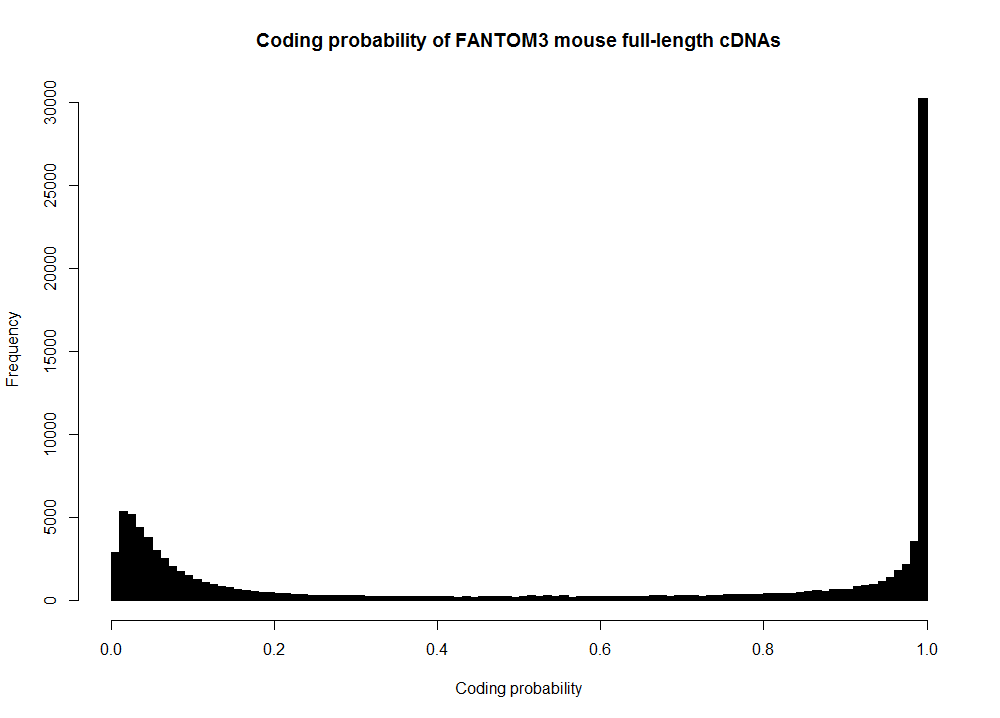
\includegraphics[width=\textwidth,natwidth=1000,natheight=718]{fantom3_coding_probability.png}
   \caption[Coding probability of FANTOM3 mouse cDNAs]{Distribution of coding probabilities of FANTOM3 mouse full-length cDNAs as predicted by CPAT\cite{tang2014fantom3codingprob}.}
   \label{fig:fantom3_coding_prob}
\end{figure}

\subsection{Non-coding RNAs}

Half of interrogated loci harboured an open reading frame FANTOM2\cite{pmid12466851}

Diverse class of non-coding RNAs, broadly broken down into long and short non-coding RNA

Classical non-coding RNA found in both prokaryotes and eukaryotes are ribosomal RNAs and transfer RNAs, which are both involved in protein synthesis

Micro-RNAs (miRNAs) were first first observed in 1993 in Caenorhabditis elegans\cite{pmid8252621} as a small double-stranded RNA that were bound to the 3' untranslated region (UTR) of an mRNA. The binding of the miRNA inhibited the translation of the mRNA and is one of the mechanisms by which miRNAs post-transcriptionally regulate gene expression. The biogenesis of miRNAs begins with the cleavage by an enzyme called Dicer\cite{pmid11201747}, which is part of the RNase III family. miRNAs inhibit translation by recruiting a ribonucleoprotein complex called RNA-induced silencing complex (RISC). Short-interfering RNAs are also cleaved by Dicer and can also bind to mRNA but require complete complementarity. MiRNAs are products of dsRNAs encoded in genes in our genome and do not require full complementarity to bind to a target mRNA thus one miRNA may regulate several genes.

A single-stranded nucleic acid molecule will tend to fold up on itself to form localised double-stranded regions, producing structures called hairpins or stem-loop structures. This is due to the hydrophobic nature of the bases, which means that the bases are unstable when exposed to an aqueous environment. Pairing of the bases enables them to be removed from interaction with the surrounding water and stabilising the DNA helix.

Assembly of non-coding RNAs with proteins as ribonucleoprotein (RNP) structures
Interaction of non-coding RNAs with chromatin

\section{The repetitive genome}

Discovery of repeated DNA sequences\cite{Britten1968} by measuring the reassociation rates of DNA strands.

The FANTOM and ENCODE projects demonstrated that a large percentage of the mammalian genome is transcribed, which became known as pervasive transcription\cite{pmid21765801}. Critique of ENCODE\cite{pmid23431001, pmid23479647, pmid23137679}.

Make the distinction between junk DNA and non-coding DNA.

Since the release of the draft human genome sequence\cite{venter2001sequence, lander2001initial}, it was established that only a small fraction of the genome is made up of protein-coding sequences and the majority of the genome was made up with repetitive elements. As the human genome contains the entire instruction set that is necessary for the development of a human, the decoding of the genome was thought to provide answers to many outstanding biological questions. However, there are several paradoxes that are still currently unresolved:

\begin{enumerate}
   \item K-value paradox: complexity does not correlate with the number of chromosomes
   \item C-value paradox: complexity does not correlate with genome size
   \item N-value paradox: complexity does not correlate with the number of protein coding genes
\end{enumerate}

If we measure organismal complexity in terms of mental cognition, we observe that complexity is not correlated to the number of chromosomes, the size of genomes, and the number of protein coding genes. Humans have 46 chromosomes and some species of butterflies have over hundreds of chromosomes, such as \textit{Polyommatus atlantica}. In terms of genome size, the species \textit{Polychaos dubium}, a freshwater amoeboid, has one of the largest genomes known with around 670 gb of DNA sequence; humans on the other hand have a genome size of roughly 3 gb. And lastly humans have roughly the same number of protein-coding genes as \textit{Caenorhabditis elegans}, roughly 20,000 versus 21,000, respectively. However, the \textit{C. elegans} genome is about 100 mb\cite{celegans1998sequencing}, which is approximately 30 times smaller than the human genome, despite having a similar number of genes. One of the discrepancies between genome sizes despite having a similar number of genes is due to repetitive elements, which makes up roughly 50\% of the human genome. Among 66 vertebrate genomes, the percentage coverage of repetitive elements in the human genome is quite high (Figure ~\ref{fig:repeat_coverage_vertebrate_genome}).

\begin{figure}[!ht]
   \centering
   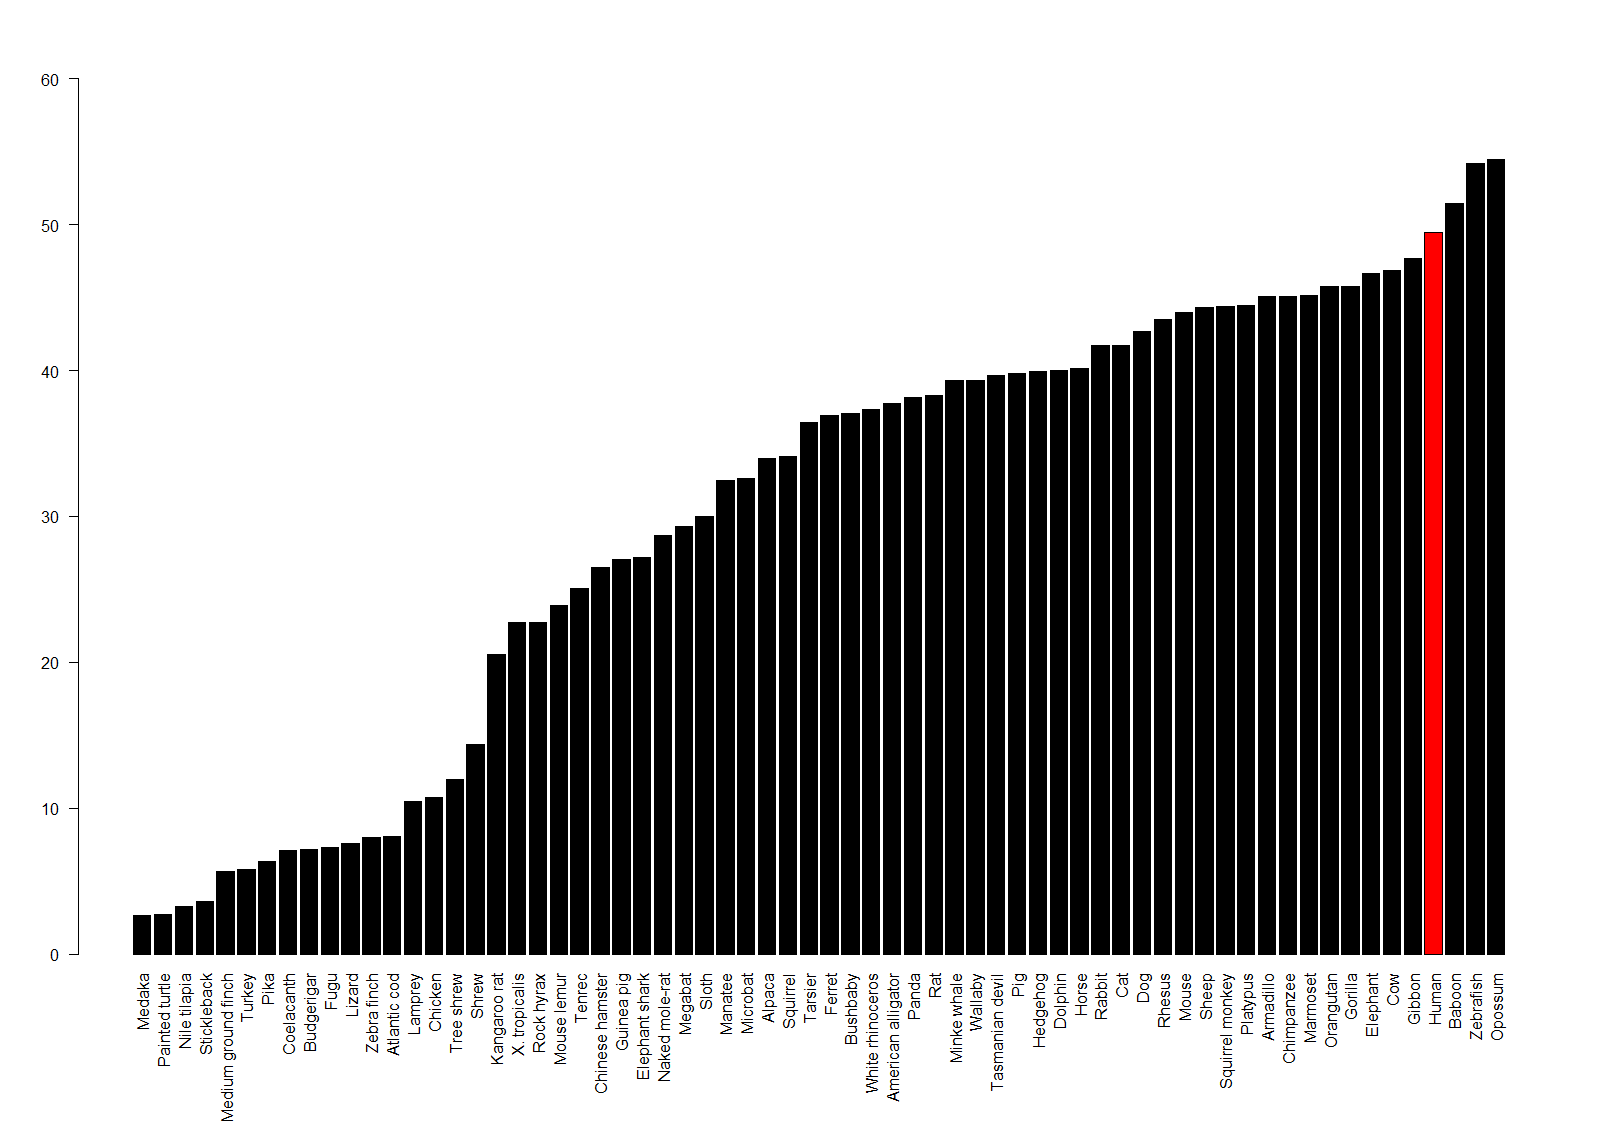
\includegraphics[width=\textwidth,natwidth=1600,natheight=1148]{repeat_coverage_vertebrate_genome.png}
   \caption[Coverage of repetitive elements in vertebrate genomes]{The total coverage of repetitive element in 66 vertebrate genomes as annotated by RepeatMasker in the respective genomes\cite{tang2014repcoverage}.}
   \label{fig:repeat_coverage_vertebrate_genome}
\end{figure}

However, the larger vertebrate genomes do not always contain the highest percentage of repetitive elements (Figure ~\ref{fig:genome_size}). At least in humans, transposons make up the majority of the repetitive elements that make up the human genome. In particular class I transposons (retrotransposons), which are able to transcribed and inserted into the genome, make up a large portion of the human genome. W.Ford Doolittle and Carmen Sapienza wrote in 1980\cite{doolittle1980selfish}: ``When a given DNA, or class of DNAs, of unproven phenotypic function can be shown to have evolved a strategy (such as transposition) which ensures its genomic survival, then no other explanation for its existence is necessary" and Leslie Orgel and Francis Crick, wrote that junk DNA has little specificity and conveys little or no selective advantage to the organism\cite{orgel1980selfish}.

The origin of the term ``junk DNA" is usually attributed to Susumu Ohno, who used it to describe pseudogenes, which are gene copies that have no known biological function. In its modern day usage, ``junk DNA" is used to describe DNA sequence that goes not play a functional role in an organism. Dr. Ohno estimated that there would be an upper limit to the number of functional loci in mammalian genomes based on mutational load and a fixed mutation rate. He predicted that mammalian genomes could not have more than 30,000 loci under selection as this would guarantee a progressive decline in fitness, leading to extinction.

The C-value paradox, junk DNA and ENCODE\cite{Eddy2012}.

\begin{figure}[!ht]
   \centering
   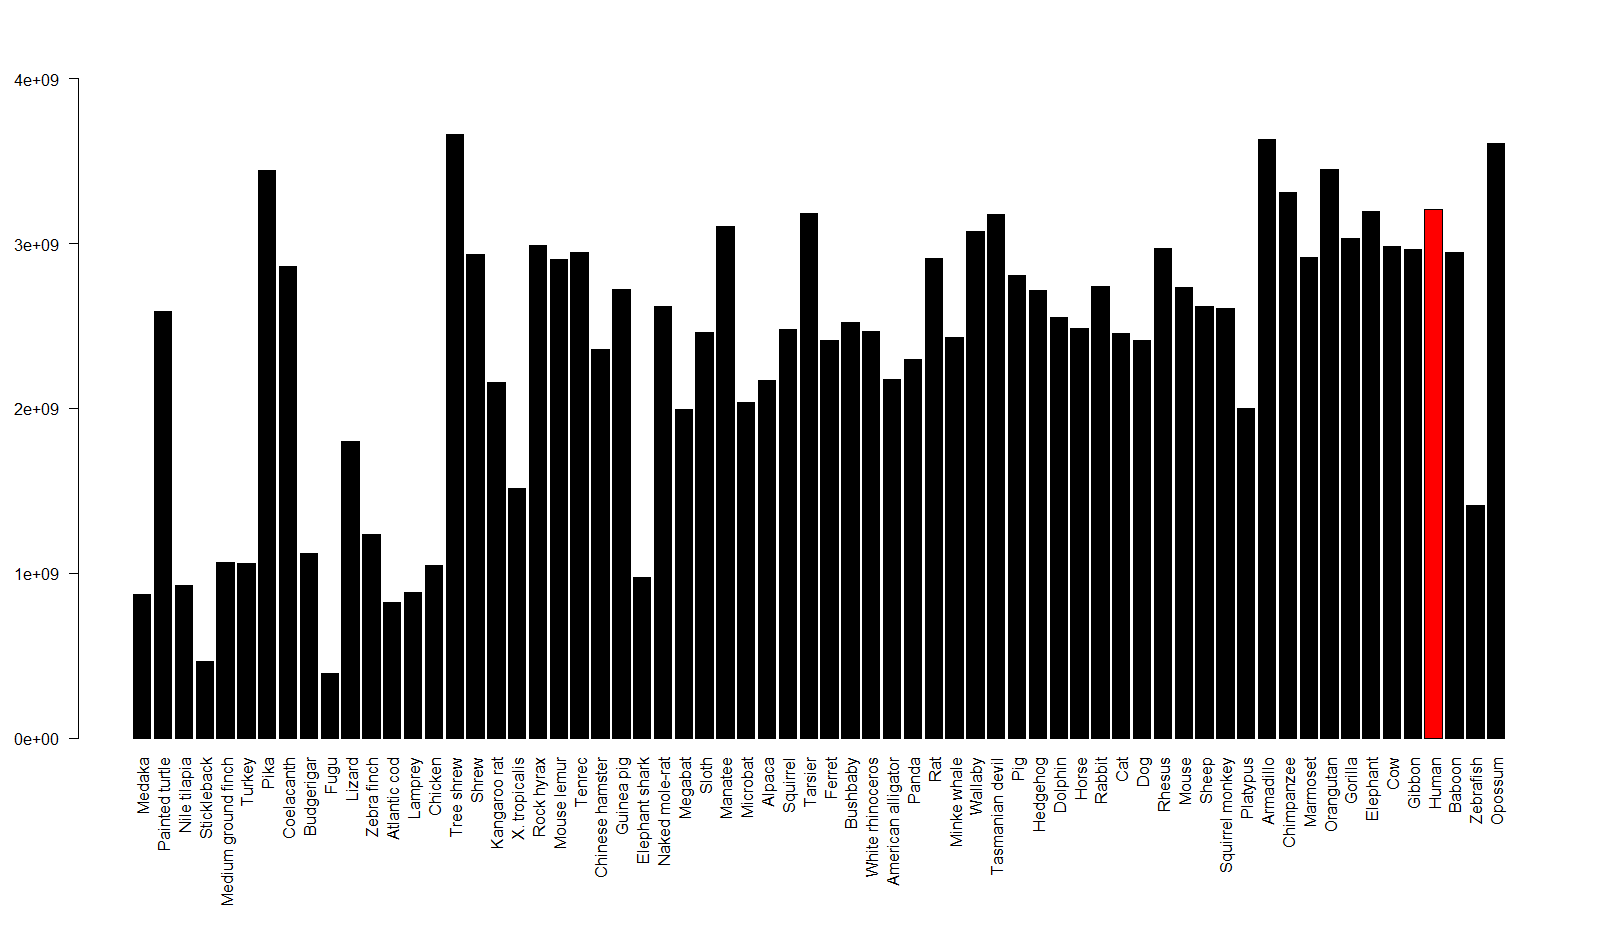
\includegraphics[width=\textwidth,natwidth=1600,natheight=932]{genome_size.png}
   \caption[Vertebrate genomes sizes]{The genome sizes of 66 vertebrate genomes, sorted from the lowest to highest percent of repetitive element coverage\cite{tang2014gensize}.}
   \label{fig:genome_size}
\end{figure}

\begin{itemize}
   \item Repeat-associated binding sites (RABS) are over-represented in proximity of regulated genes and that the binding motifs within these repeats have undergone evolutionary selection
   \item Indeed, studies conducted both at the gene and genome levels have uncovered TE insertions that seem to have been co-opted - or exapted - by providing transcription factor binding sites (TFBSs) that serve as promoters and enhancers, leading to the hypothesis that TE exaptation is a major factor in the evolution of gene regulation.
   \item The transcription of repetitive elements, especially transposable elements, in specific tissues
   \item Repetitive elements are usually highly methylated, however differentiation methylation patterns of repetitive elements was observed in specific tissues
   \item Functions of some GWAS candidates in intergenic regions (such as http://www.nature.com/nature/journal/v507/n7492/full/nature13138.html)
   \item The regulated retrotransposon transcriptome of mammalian cells\cite{pmid19377475}
\end{itemize}

\section{Stem cells}

The existence of stem cells was discovered in 1961 and the stem cell theory was published in 1963\cite{pmid13970094}. In this work, Canadians researchers James Till and Ernest McCulloch proved that stem cells were present in bone marrow. They exposed mice to high doses of radiation that killed off the mouse's blood and immune forming system and then injected bone marrow cells into some of the mice. The mice that didn't receive the transplants died and the mice that received the transplants survived because the bone marrow cells rebuilt their blood and immune forming systems. The bone marrow cells were able to reproduce themselves as well as generating different cell types. Human bone marrow transplants are still routinely used nowadays to treat leukaemia and other kinds of blood disorders.

Stem cells have two key characteristics that differ from other cells: they can reproduce themselves for long periods of time, known as self-renewal, and they can differentiate or specialise into specific cell types under certain conditions. What Till and McCulloch discovered were actually adult or tissue stem cells (ASCs), which are multipotent; this means that they have limited differentiation ability and are only able to generate specific types of differentiated cells. For example, haematopoietic stem cells, which are a type of adult stem cells that reside in the medulla of the bone (bone marrow), are only able to give rise to different mature blood cell types and tissues. In 1981, researchers were able to derived embryonic stem cells (ESCs) from mouse embryos (specifically the inner cell mass of blastocysts) and grow them on Petri dishes\cite{pmid7242681, pmid6950406}. In normal development, the inner cell mass begins growing into all the different cell types of the fully developed body and as such ESCs are able to differentiate into all the cell types that make up the body and they are pluripotent. Cells with the highest potency or with the most differentiation potential, are known as totipotent cells and are able to form all the cell types in a body, including the placental cells. Embryonic cells within the first couple of cell divisions after fertilisation are the only cells that are totipotent.

In 2006, a new methodology was invented by Takahashi and Yamanaka to generate another type of stem cell, called induced pluripotent stem cells (iPSCs)\cite{pmid16904174}. In their work, they discovered a way to generate pluripotent stem cells from somatic cells, which have no differentiation potential. Since their discovery, many researchers wondered about the development potential of iPSCs and in 2009 a Chinese group were successful in creating a live mice from iPSCs that were able to produce offspring\cite{pmid19672241}. In one of the first studies to show the clinical application of human iPSCs to human disease, a team derived iPSCs from fibroblasts of patients suffering from alpha 1 antitrypsin deficiency, corrected the disease causing mutation, and used the corrected stem cells to produce liver cells that were transplanted into the liver via intrasplenic injection\cite{pmid21993621}. Since the cells are genetically identical to the patient, there is no worry about rejection or immune problems, and is one reason why iPSCs are an attractive option for regenerative medicine.

\section{The role of bioinformatics in genomics}

Modern day high-throughput sequencers generate large amounts of data; for example in the blood transcriptome project (Chapter 7), one lane of sequencing on the HiSeq2000 produced 74.5 million reads (using 15 gigabytes of storage space when uncompressed). To deal with data at this scale, informatics tools for storing, managing, and analysis such data sets are absolutely necessary. Bioinformatics can be thought of as informatics for biological data, though historically it was defined as ``the study of informatic processes in biotic systems"\cite{pmid21483479}. The HGP was one of the first large scale international research efforts and bioinformatics was crucial towards the successful completion of the HGP\cite{stein1996perl}. An important principle established during the HGP, called the ``Bermuda Principles", was set by an international assortment of genome-research leaders towards the rapid and public sharing of human genome information. These set of commitments left a lasting legacy in large genomic science projects such as The International HapMap Project, ENCODE and modENCODE, and The Cancer Genome Atlas where data was made freely available prior to publication\cite{contreras2011bermuda}. The public availability of data from these projects have resulted in major advances in genomics and bioinformatics.

The FASTQ format was formally defined in 2010\cite{pmid20015970} and has become the \textit{de facto} format for storing raw sequencing output. FASTQ is similar to the FASTA format with the addition of storing quality scores for each nucleotide. The format is simplistic, which may be the reason for its popularity before being formalised. The establishment of a standard format is important as developers can produce programs, such as sequence aligners, that can process output from different sequencing machines. Another standard file format for storing sequence alignments is the Sequence Alignment/Map (SAM) format\cite{pmid19505943}.

The reads generated from the second generation of sequencers were much shorter and much more numerous than traditional Sanger sequencing reads. The Illumina GAII can produce up to 100 million reads of 50 bp in a single run. Traditional sequence alignment tools using the Needleman–Wunsch algorithm or Smith–Waterman algorithm were simply too slow and new developments were necessary. The popular short-read alignment tool, BWA\cite{pmid19451168}, implements the Burrows–Wheeler transform to deal with millions to billions of short reads. The Burrows-Wheeler transform allows a large mammalian genome, for example human, to be indexed and stored efficiently into memory\cite{pmid19430453}.

Comparing genomic features using BEDTools\cite{pmid20110278}.

Expression data sets are commonly stored as matices; for example if we let $A$ be an $m \times n$ matrix, where $a_{ij}$ are elements of $A$, the $i^{th}$ row would represent the transcriptional response of the $i^{th}$ gene and the $j^{th}$ column would represent the expression profile of the $j^{th}$ assay:

\begin{align*}
   A = \begin{bmatrix} a_{11} & \cdots & a_{1j} & \cdots & a_{1n} \\
   . && . && . \\
   a_{i1} & \cdots & a_{ij} & \cdots & a_{in} \\
   . && . && . \\
   a_{m1} & \cdots & a_{mj} & \cdots & a_{mn} \end{bmatrix}
\end{align*}

A differential expression analysis can be easily performed on an expression matrix, such as by using the edgeR package\cite{pmid19910308} from Bioconductor\cite{pmid15461798}. Multidimensional scaling methods, such as Singular Vector Decomposition (SVD), can also be applied on the matrix to find underlying patterns in the data. A very popular visualisation method of expression data is the use of heatmaps that reflect the relative expression strength of each element in the matrix ($a_{mn}$), which is commonly used in tandem with hierarchical clustering. Co-expression matrices can be further derived from the expression matrix to find transcripts with a similar transcriptional response or assays with similar expression profiles. Networks or graphs can be built from such co-expression matrices for visual purposes or for analysing the structure of co-expression patterns.



\chapter{Template switching artefacts}\label{template_switching}
\fancytab{Chapter ~\ref{template_switching}}{\tabSpace*\thechapter}
In this work, we studied the transcriptional landscape in whole blood using a technology called nano Cap Analysis Gene Expression (nanoCAGE). While it was expected that the variability between samples would be high due to the heterogeneous nature of whole blood, unexpectedly, samples prepared with the same or similar barcodes had very similar expression profiles regardless of biological origin. This affected differential expression analyses whereby the estimation of variability was increased due to biological replicates having very different expression profiles. In order to adjust for the barcode bias, we identified template-switching artefacts that caused the bias, and developed a bioinformatic solution for removing these artefacts and improved the nanoCAGE protocol to mitigate the barcode bias. This work laid the groundwork for analysing transcriptome profiling using high-throughput sequencing, by understanding how technical artefacts and biases are able to form and affect downstream analyses.

%to include page styles in pdf, pagecommand=\thispagestyle{plain}
\includepdf[pages={-}, lastpage={12}]{paper/barcode_bias.pdf}

\chapter{Role of small RNAs in DNA damage repair}\label{ddrna}
\fancytab{Chapter ~\ref{ddrna}}{\tabSpace*\thechapter}
It has been previously reported that small RNAs play a role in establishing the DNA damage response\cite{pmid19444217}. We leveraged the discovery potential of small RNA sequencing to gain some insight into the potential interplay between small RNAs and DNA damage. Intriguingly, we discovered that small RNAs formed near the site of DNA damage. We considered alternative hypotheses that could explain the presence of these small RNAs such as RNA degradation or technical artefacts. We\footnote{All the bioinformatic analysis was performed by Dave Tang.} characterised certain features of the DNA damage small RNAs (DDRNAs) to the population of sequenced small RNAs and observed that the bulk of the DDRNAs had a characteristic size and nucleotide profile, suggesting that they are not random degradation products. Furthermore, we performed experiments to suggest possible biogenesis pathways and the knock-down of Dicer and Drosha, which are enzymes involved with small RNA processing, affected the profile of DDRNAs and impaired the DNA damage response. This work has important implications to the observation that the genome is pervasively transcribed, as it offers a hypothesis that pervasive transcription is necessary for maintaining DNA integrity.

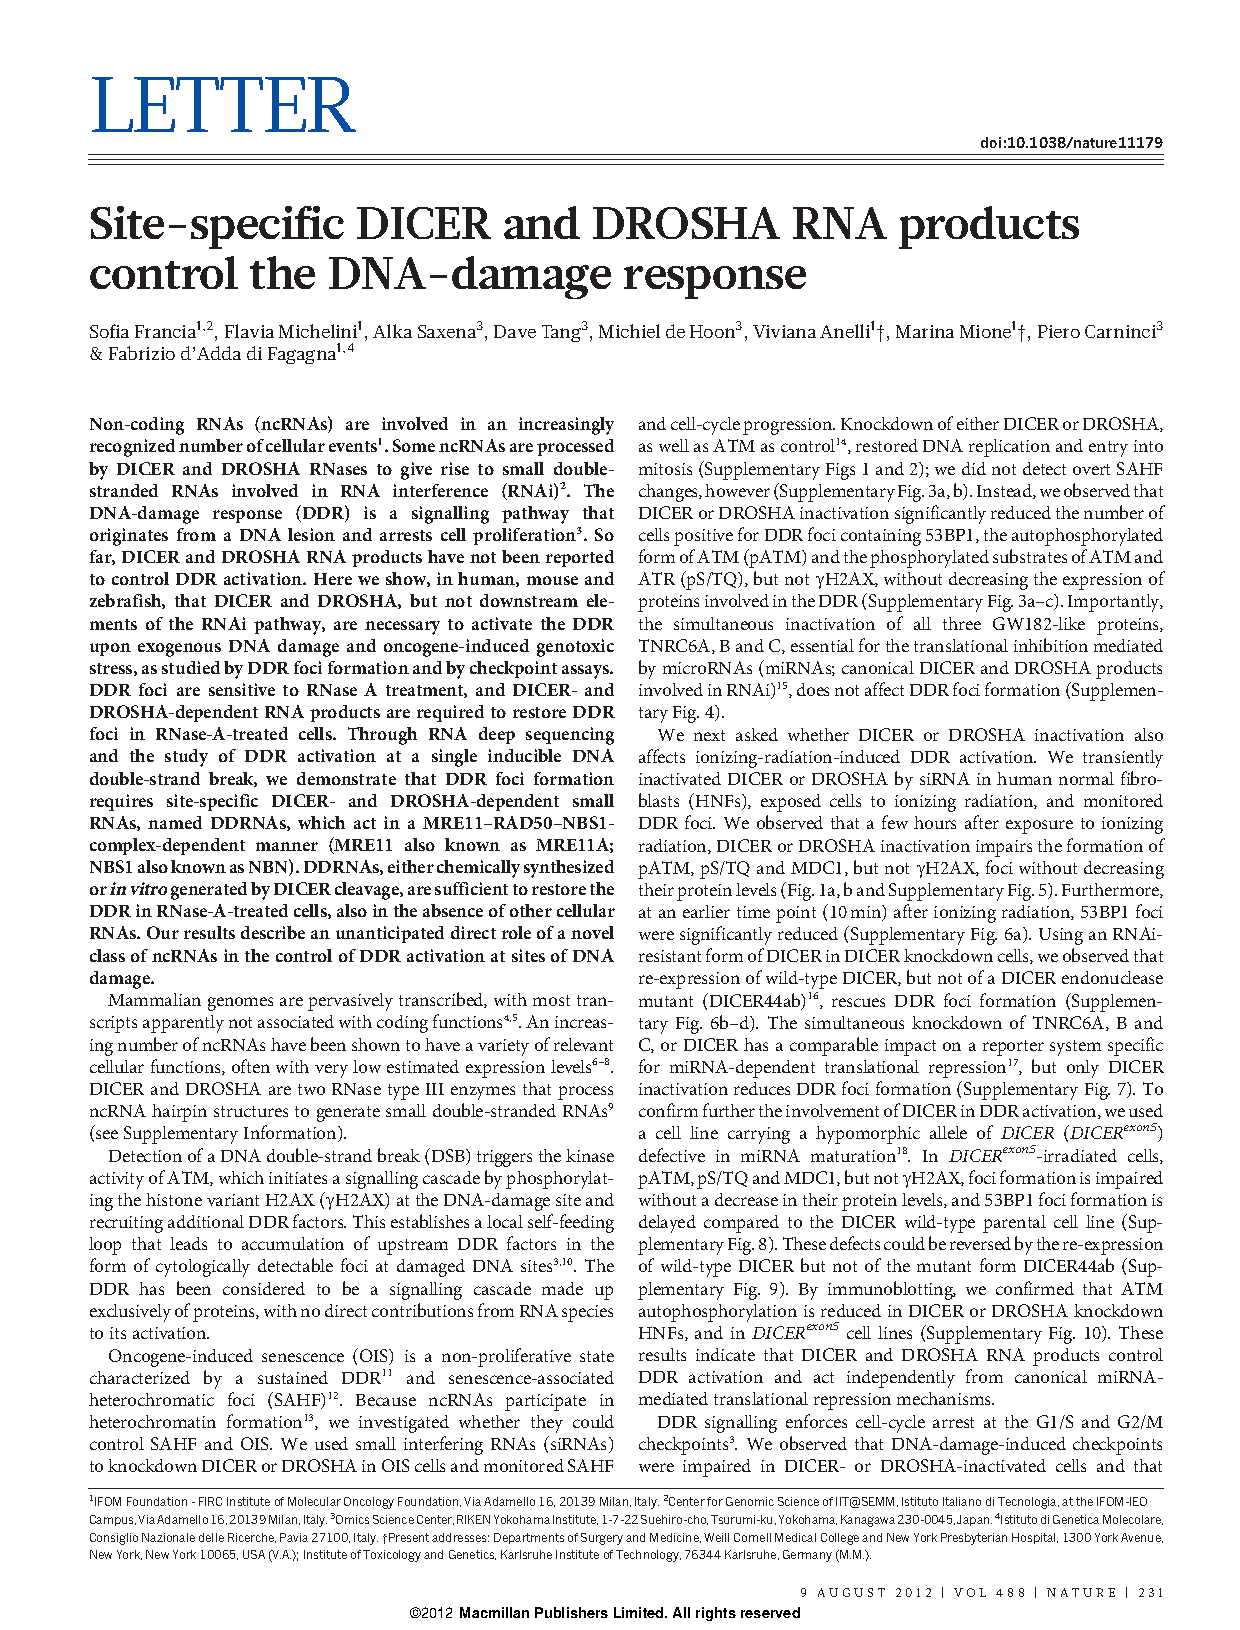
\includepdf[pages={-}, lastpage={8}]{paper/ddrna.pdf}

\chapter{Rett syndrome and piRNAs}\label{pirna}
\fancytab{Chapter ~\ref{pirna}}{\tabSpace*\thechapter}
Mutations in the gene methyl CpG binding protein 2 (MECP2) are the cause of most cases of Rett syndrome (RTT), a neurodevelopmental disorder that affects girls almost exclusively. Given that the MECP2 protein contains a methyl-CpG binding domain (MBD) and can recruit histone deacetylases, they are largely considered as transcriptional repressors. In rodents, the absence of MeCP2 leads to an increase in long interspersed nuclear elements-1 (L1) neuronal transcription and retrotransposition \citep{pmid21085180}. Furthermore, by analysing neuronal progenitor cells (derived from fibroblasts using induced pluripotent stem cell technology) and post mortem human tissues from patients with RTT, it was revealed elevated L1 activity compared \citep{pmid21085180}. MeCP2 chromatin immuno-precipitation sequencing in mice whole brain also suggested that MeCP2 may play a role in silencing retrotransposons \citep{pmid20188665}. A class of small RNAs called piwi-interacting RNAs (piRNAs), can be derived from L1 elements, and are involved in silencing transposons, by forming the piRNA-induced silencing complex (piRISC). In this work, we\footnote{All the bioinformatic analysis was performed by Dave Tang; details of the analysis can be found at \url{https://github.com/davetang/22976001}.} analysed a short RNA library prepared from cerebellum of mice with a Mecp2 knock-out \citep{pmid20921386}. Our analyses revealed that hundreds of piRNAs are expressed in the cerebellum, including previously characterised brain-specific piRNAs. Furthermore, we found that in the Mecp2 knock-out mice, a large number of piRNAs were over-expressed, suggesting that piRNA expression levels may also be affected by the absence of Mecp2. While piRNAs are thought to function mainly as silencers for transposons in germ cells, this study suggests that a subset of piRNAs may have other roles in gene regulation.

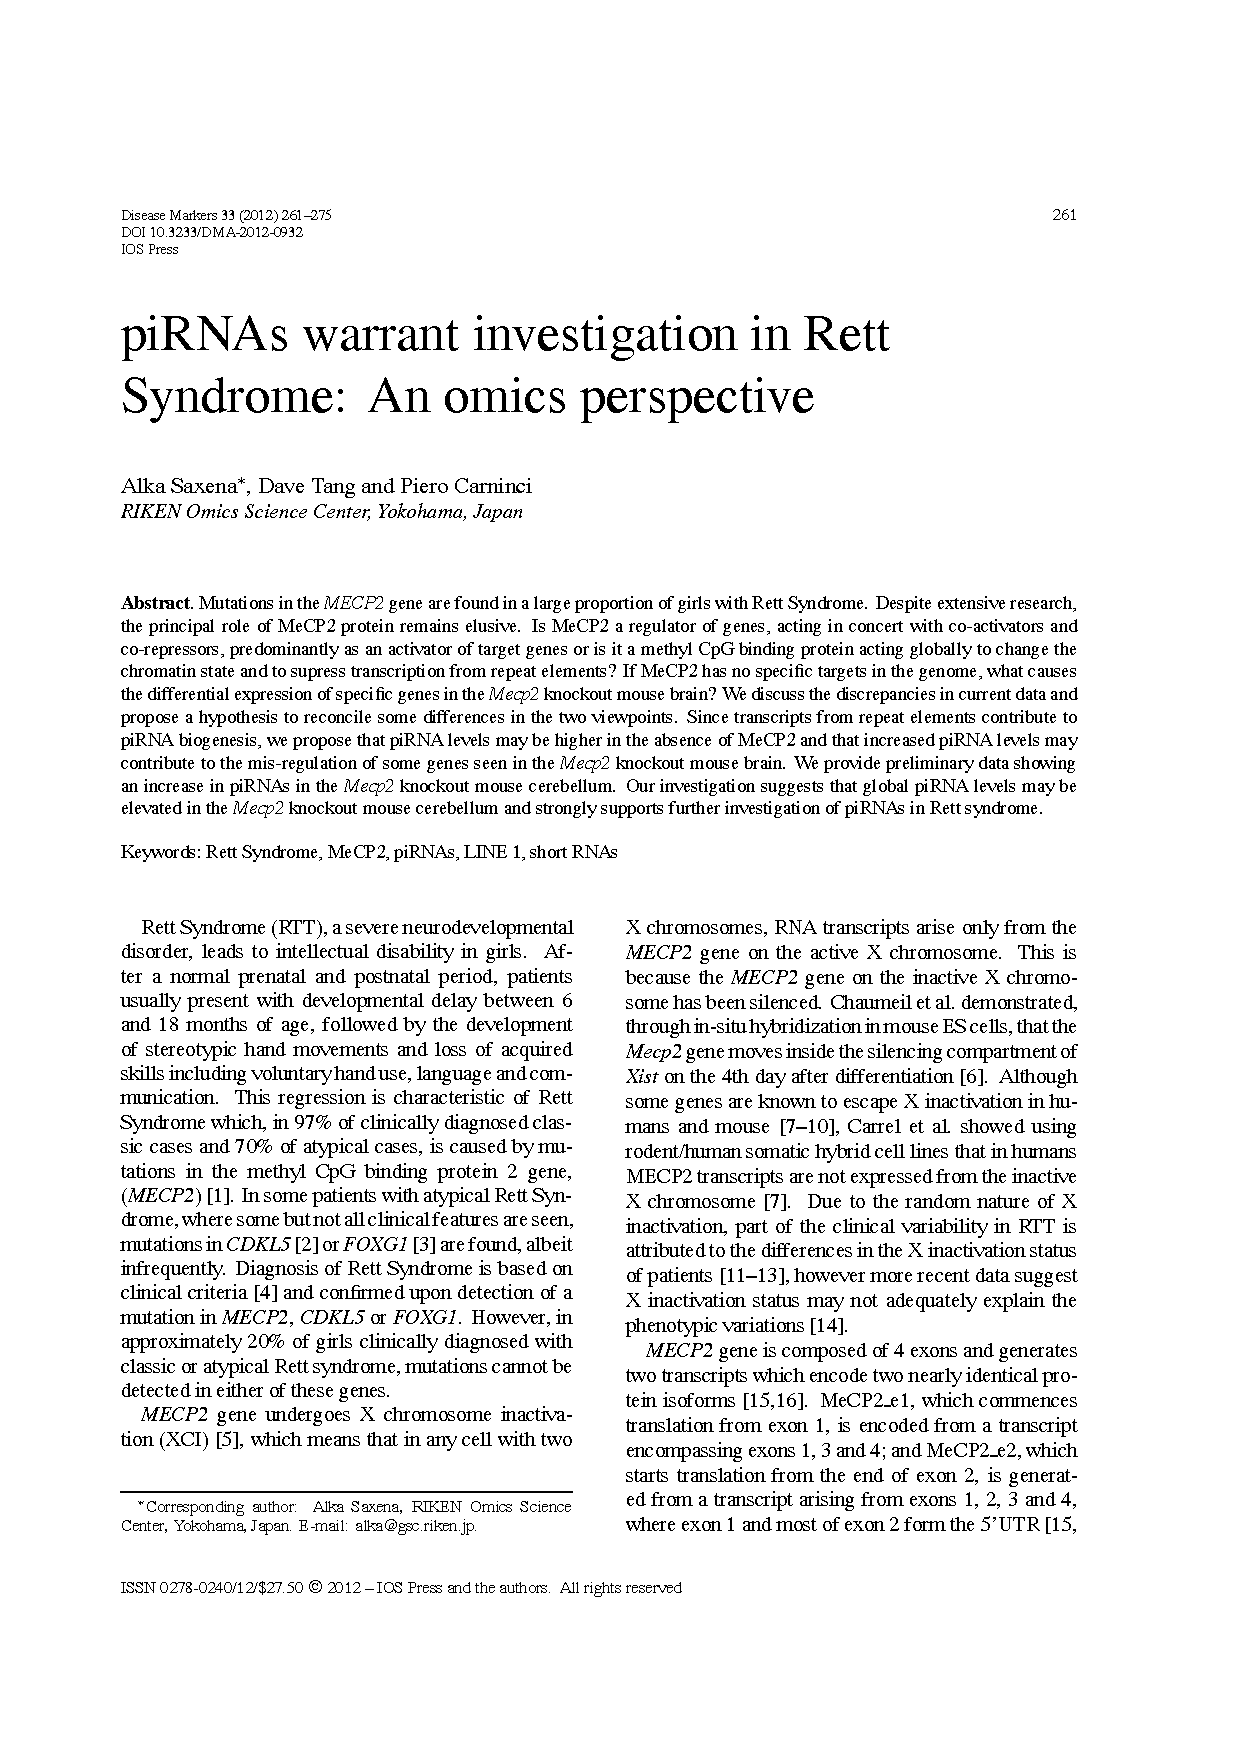
\includepdf[pages={-}, lastpage={8}]{paper/pirna.pdf}

%\chapter{CCL2 activates hypoxia related genes}\label{ccl2}
%\fancytab{Chapter ~\ref{ccl2}}{\tabSpace*\thechapter4}
%\input{chapter/ccl2}
%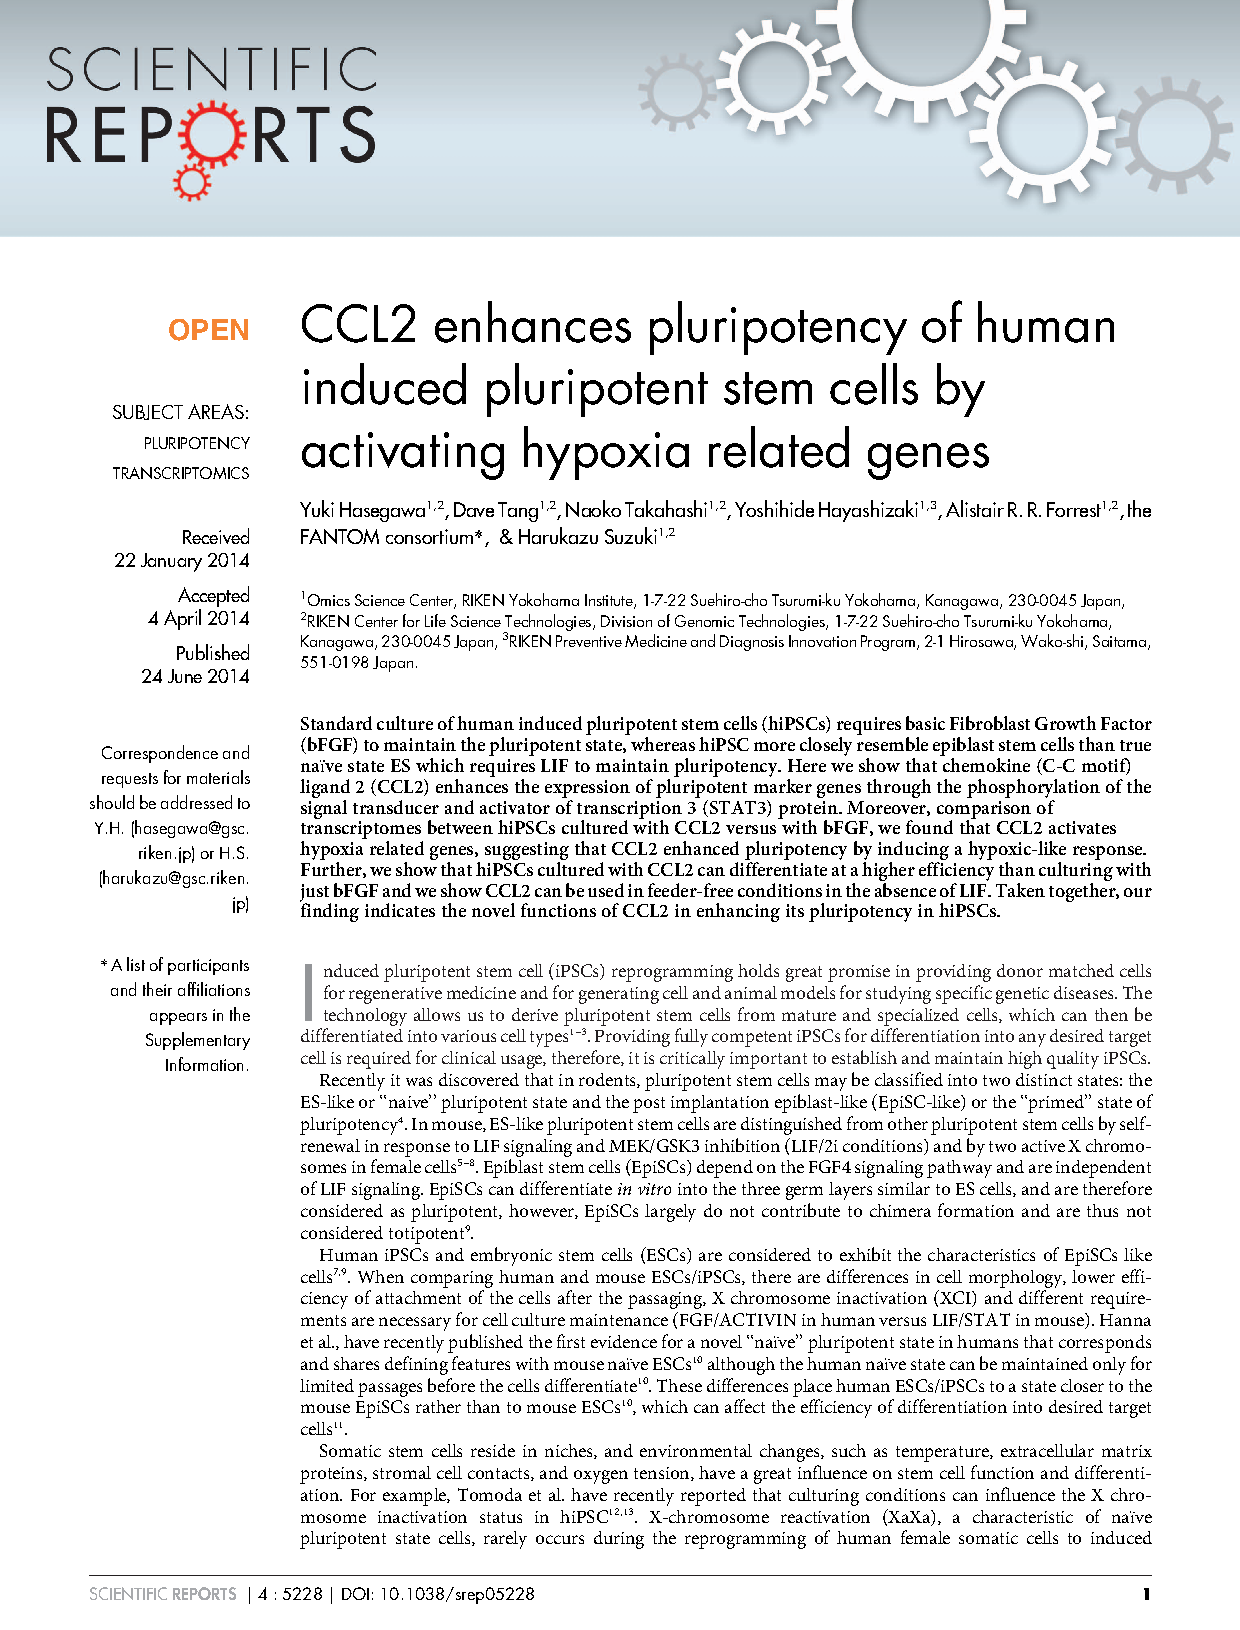
\includepdf[pages={-}, lastpage={9}]{paper/ccl2.pdf}

\chapter{Regulated expression of repetitive elements}\label{repeat}
\fancytab{Chapter ~\ref{repeat}}{\tabSpace*\thechapter4}
It is well established that the human genome is pervasively transcribed and this has been attributed to a ``leaky" transcriptional system. Our observation that small RNAs are formed near the vicinity of DNA damaged sites and are required for establishing the DNA damage response, implies that all RNAs are potentially useful, since any site in the genome is vulnerable to DNA damage. A class of RNA that is often neglected from study are those that form from the repetitive portion of the genome. It is estimated that at least half of the human genome is made up of repetitive elements (REs) and transcription initiation has been observed within these elements \citep{pmid19377475}. However, the general impression is that these elements are non-functional and are simply transcriptional noise. Motivated by the hypothesis that all RNAs could be potentially useful, we quantified and catalogued expression signal from REs using the FANTOM5 atlas.

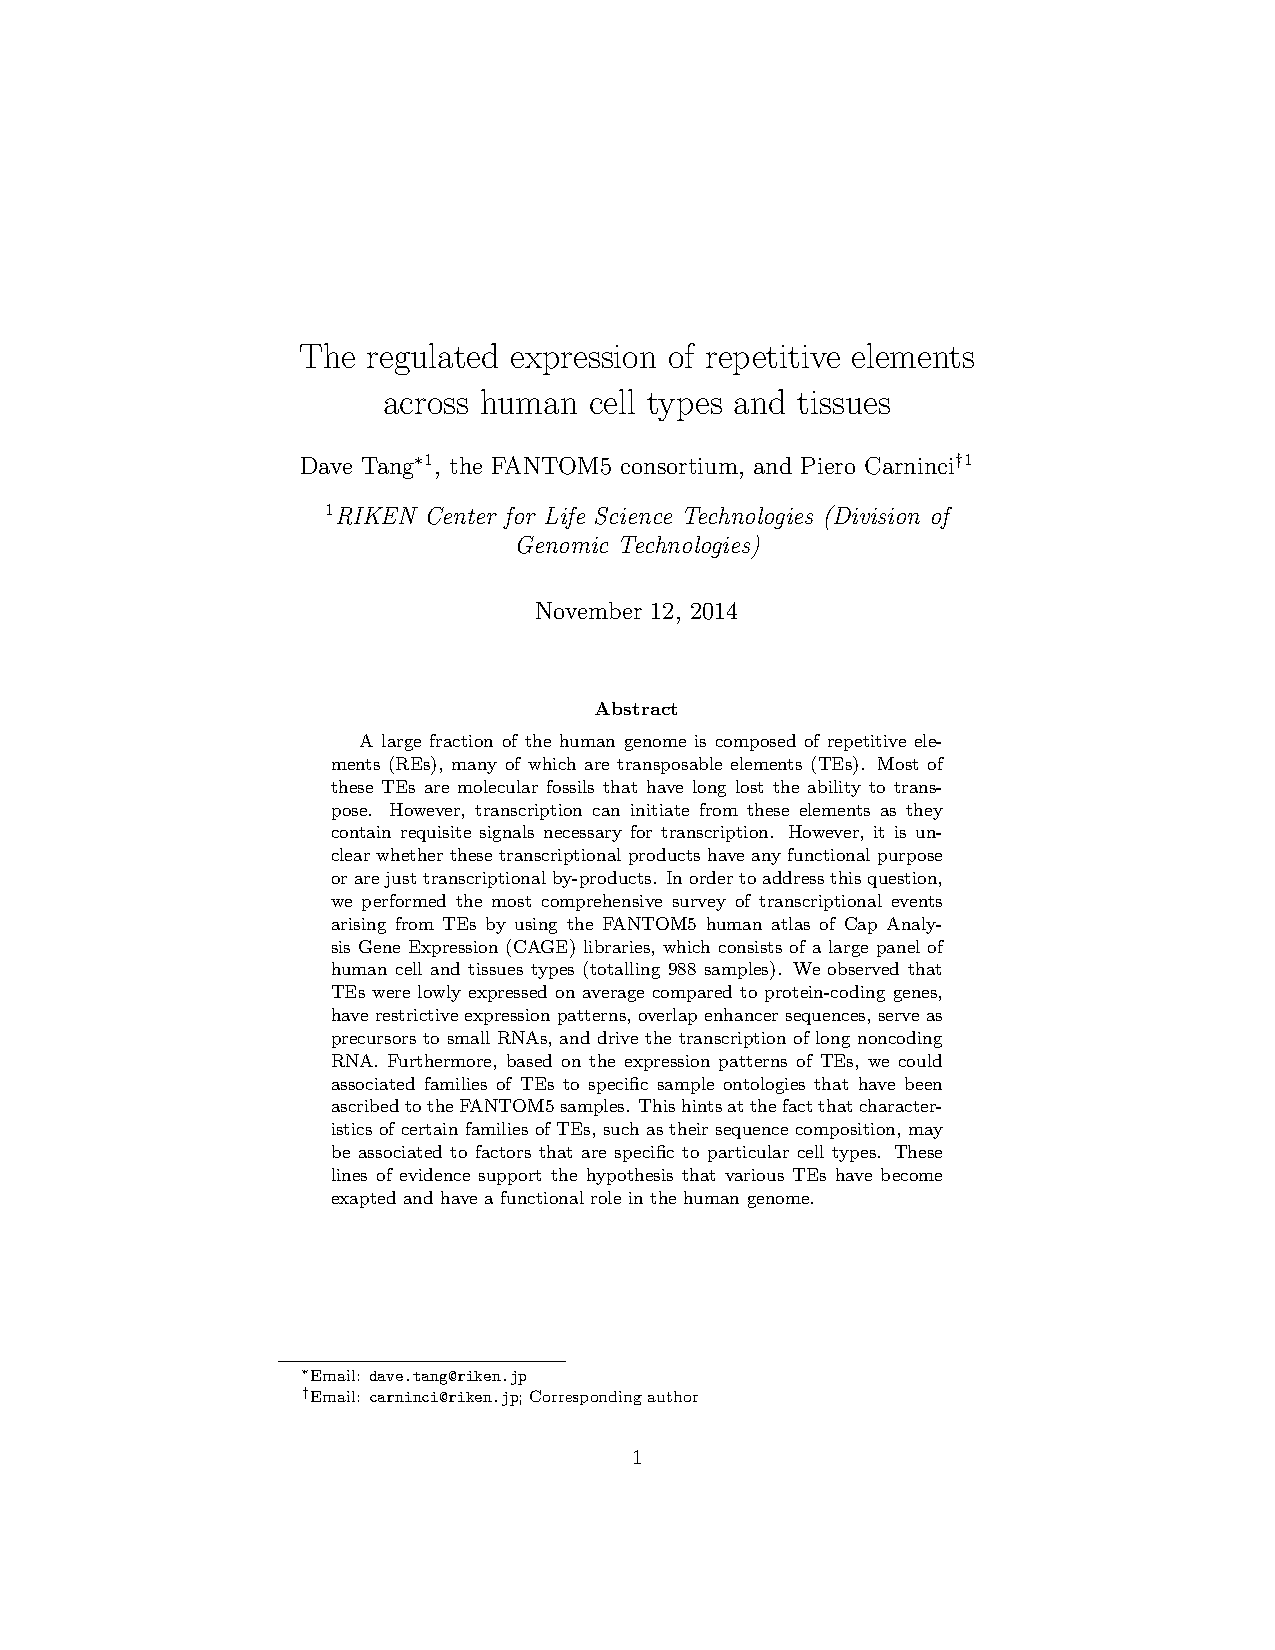
\includepdf[pages={-}, lastpage={21}]{paper/repeat.pdf}

%\chapter{The blood transcriptome}\label{blood}
%\fancytab{Chapter ~\ref{blood}}{\tabSpace*\thechapter}
%\input{chapter/blood}

\chapter{General discussion}\label{discussion}
\fancytab{Chapter ~\ref{discussion}}{\tabSpace*\thechapter}
\setlength{\parskip}{\baselineskip}%
\setlength{\parindent}{0pt}%

Small non-coding RNAs have been implicated in many biological processes, such as messenger RNA regulation or transposon silencing. We identified a role of small non-coding RNAs in the DNA damage repair mechanism. The inactivation of dicer and drosha, which are required for the biogenesis of small RNAs, leads to a loss of DNA damage repair. We sequenced the small RNAs from cells that had induced DNA damage and found small RNAs arising from the vicinity of the DNA double-strand break. Importantly, synthetic small RNAs mimicking these small RNAs could drive the DNA damage response \cite{francia2012site}.

Parkinson’s disease (PD) is a slowly progressive disease in which dopamine neurons in the substantia nigra degenerate undetected for years before clinical symptoms develop. The lack of clinical symptoms highlights the necessity of a laboratory test, such as an assay for biomarkers, which can correlate subjects with PD risk. We have profiled the RNAs in the whole blood sample of PD patients and age-matched controls using high-throughput deepCAGE sequencing. By comparing the RNA profiles between PD patients and controls, we aim to discover novel biomarkers that are present in whole blood, which may be further developed into a non-invasive clinical test for PD.

\begin{itemize}
   \item Are the majority of detected low-level transcription due to technical artifacts and/or background biological noise?
   \item Sequencing depth and sampling of RNA molecules; absolute transcript quantification will help (such as using unique molecule identifiers and non-PCR based methods)
   \item Functional transcriptomics in the post-ENCODE era, specifically what is the criteria for functionality
   \item The technologies that allowed full length cDNA sequencing
   \item PacBio sequencing has read lengths greater than 10kb and can be used for full length cDNA sequencing
\end{itemize}

\subsection{Experimental differences}

Starting RNA amount required by different protocols and it may not be possible obtain sufficient amounts of starting material. Thus PCR-based techniques are popular and are able to amplify RNA isolated from single cells. This leads to less heterogeneity compared to techniques that pool cells, which may have very different expression profiles. It is important to obtain a true profile of transcription in cells.

DNA sequences do not exist as naked DNA \textit{in vivo}, but are usually packaged in higher order DNA structures thus \textit{in vitro} models may not recapitulate the entire story.

poly-A versus random primers
cytoplasmic versus nuclear enrichment
CAGE versus RNA-seq

\subsection{Signal versus noise}

The primary aim of transcriptomics is to capture the expression patterns of the full set of transcripts in a cell or tissue. However, technical and biological variances cause fluctuations in the measurements, which is referred to as noise. Technical variation may result from the sequencing technology and from carrying out the experimental protocol; this type of noise is predictable and follows a Poisson distribution. Biological variation arises from the natural variability in different biological entities; this variation can be small for genetically identical samples or can be very large, such as in a heterogeneous sample such as blood. Biological variation may be due to biological processes that are not perfect such as noisy splicing, which increases the mRNA isoform diversity in human cells\cite{pmid21151575}. Other sources of noise may be from contamination, such as from genomic DNA.

The random sampling of lowly expressed versus highly expressed transcripts.

Expression profiles from sample of cells versus single cell.

\subsection{Coding versus non-coding transcripts}

Transcripts of Unknown Function (TUFs)
The role of non-coding RNAs
The role of repetitive elements in the genome

\subsection{Transcriptome profiling using CAGE}

Unbiased profiling of total transcripts
Comparison with different environmental conditions
Gene ontology enrichment


\chapter*{Acknowledgements}
\epigraph{``Twenty years from now you will be more disappointed by the things that you didn't do than by the ones you did do. So throw off the bowlines. Sail away from the safe harbor. Catch the trade winds in your sails. Explore. Dream. Discover."}{--- \textup{Mark Twain}}

The culmination of work presented in this thesis would not have been possible without the guidance and support of many friends and colleagues. But my involvement in this PhD project would not have even begun if not for my supervisor who accepted me into the program and a former colleague who forwarded the opening to me. I still remember the predicament I faced over 4 years ago when I had to decide whether or not I would commit to the idea of potentially working in Japan. I had already brushed off the idea once but in the end I was convinced that it was a tremendous opportunity and I would have regretted it if I let it slip by. In the end, I decided to set my sails to explore an entirely new world.

To this day, I have absolutely no regrets for embarking on this journey and it has been the best experience of my life (thus far). I had to leave behind close friends of many years but I still remember their responses when I asked for their advice regarding the opportunity in Japan. Their answers were unanimous; clearly, they had had enough of me. I've made many new friends in Japan and I'd like to think that they know who they are. Thanks guys and gals for enduring me! I would also like to acknowledge the Good Samaritans who answer questions on discussion forums and mailing lists; where would I be without them.


%\bibliographystyle{plainnat}
\bibliographystyle{unsrtnat}
\bibliography{bibliography/reference}

\end{document}
